\documentclass[11pt,letterpaper]{article}
\usepackage[utf8]{inputenc}
\usepackage[T1]{fontenc}
\usepackage{lmodern}
\usepackage[spanish,es-nodecimaldot]{babel}
\usepackage[margin=2.2cm]{geometry}
\usepackage{graphicx,float,booktabs,longtable,array,enumitem,amssymb}
\usepackage[hidelinks]{hyperref}
\usepackage{xcolor,fancyhdr}
% Permite compilar desde la carpeta del documento, entregables o el proyecto.
\graphicspath{{../img/}{img/}{entregables/img/}{../../img/}{../../entregables/img/}{../entregables/img/}}
\setlength{\parskip}{4pt}\setlength{\parindent}{0pt}
\pagestyle{fancy}\fancyhf{}
\fancyhead[L]{MINE-4214 · Proyecto Entrega 1}\fancyhead[R]{CupiTaller · Universidad de los Andes}
\fancyfoot[C]{\thepage}
\setcounter{secnumdepth}{2}

\setlength{\headheight}{14pt}
\addtolength{\topmargin}{-2pt}

\begin{document}
\begin{center}
{\Large\bfseries Proyecto · Entrega 1\\[2pt] Reservas y satisfacción en CupiTaller}\\[8pt]
MINE-4214 Modelado y Diseño de Datos\\
Universidad de los Andes · Octubre de 2026\\[6pt]
\textbf{Integrantes:} \emph{María Alejandra Pérez Petro}, \emph{Santiago Martinez Novoa}
\end{center}
\tableofcontents
\bigskip


\section{Objetivo y análisis requeridos}

\subsection{Organización y dependencia}

La \textbf{Universidad de los Andes} es una universidad privada de Bogotá, Colombia. Su \textbf{Departamento de Ingeniería de Sistemas y Computación} (DISC), dentro de la Facultad de Ingeniería, ofrece el servicio de tutorías \textbf{CupiTaller} para los cursos de programación de los primeros semestres:

\begin{itemize}[leftmargin=1.5em,itemsep=2pt]
\item \textbf{Introducción a la Programación} (código ISIS-1221, abreviado \textbf{IP}).
\item \textbf{APO 1} y \textbf{APO 2}, cursos de programación que IP reemplazó. Aparecen en los datos históricos.
\item \textbf{Estructuras de Datos y Algoritmos} (\textbf{EDA}).
\item \textbf{Diseño y Programación Orientada a Objetos} (\textbf{DPOO}).
\end{itemize}

En CupiTaller, \textbf{monitores} (estudiantes que actúan como tutores de sus compañeros) atienden sesiones con cita previa. Hay tres \textbf{modalidades} de tutoría:

\begin{itemize}[leftmargin=1.5em,itemsep=2pt]
\item \textbf{Normal:} dura 50 a 60 minutos.
\item \textbf{Express:} dura 20 a 30 minutos y sirve para dudas puntuales.
\item \textbf{Normal pico:} es una sesión Normal en las semanas de más demanda.
\end{itemize}

Las citas se gestionan en \textbf{Bookeau}, la plataforma web de reservas. El estudiante pide una franja horaria. Si no hay cupo, queda \textbf{en cola}, es decir, en lista de espera, y no recibe cita; si luego consigue una reserva, la solicitud en cola se cierra con el estado «Cola cancelada por reservación». Cada cita termina en uno de estos \textbf{estados}:

\begin{itemize}[leftmargin=1.5em,itemsep=2pt]
\item \textbf{Atendida:} la tutoría se dio. Bookeau la registra como «Finalizada» o «Realizada», dos etiquetas que el proyecto trata como una sola; las reservas que quedaron abiertas se clasifican con la regla R07 (ver las reglas de negocio en la sección 1.3).
\item \textbf{Cancelada:} el estudiante canceló. Puede ser a tiempo, con excusa, por sanción, o tarde y sancionada. Una \textbf{sanción} es una penalización por incumplir las reglas de reserva.
\item \textbf{No asistió:} el estudiante no se presentó. También se clasifican así las reservas que quedaron abiertas sin llegada o sin prestador (regla R07).
\end{itemize}

Antes de la cita, el estudiante responde una \textbf{encuesta previa} (objetivo de la sesión y aceptación de condiciones). Después, responde una \textbf{encuesta de satisfacción} con una calificación de 1 a 5 al tutor y comentarios abiertos.

Cada semestre la coordinación define las franjas de atención (día y hora). Bookeau resume, por franja y semestre, cuántas reservas se atendieron, se cancelaron o no asistieron, cuántas solicitudes están o estuvieron en lista de espera y cuántos cupos hay reservados y disponibles. Es el reporte de \textbf{horarios}, que da la oferta de tutorías.

Trabajamos con dos áreas del DISC. La \textbf{coordinación de CupiTaller} planea las franjas y asigna monitores cada semestre. La \textbf{coordinación académica de los cursos} se encarga de la formación de los monitores.

\subsection{Proceso que genera los datos}

Los dos análisis usan datos que nacen de un mismo proceso: el ciclo de una tutoría en Bookeau. La tabla indica, paso a paso, quién actúa, qué ocurre y qué dato queda registrado. Los nombres entre comillas son los de las columnas tal como vienen de Bookeau.

\begingroup
\small
\setlength{\tabcolsep}{4pt}
\renewcommand{\arraystretch}{1.15}

\begin{longtable}{
>{\raggedleft\arraybackslash}p{\dimexpr 0.0495\textwidth-2\tabcolsep\relax}
>{\raggedright\arraybackslash}p{\dimexpr 0.1280\textwidth-2\tabcolsep\relax}
>{\raggedright\arraybackslash}p{\dimexpr 0.3086\textwidth-2\tabcolsep\relax}
>{\raggedright\arraybackslash}p{\dimexpr 0.3086\textwidth-2\tabcolsep\relax}
>{\raggedright\arraybackslash}p{\dimexpr 0.2053\textwidth-2\tabcolsep\relax}
}
\toprule
\textbf{Paso} &
\textbf{Quién actúa} &
\textbf{Qué ocurre} &
\textbf{Dato que queda registrado} &
\textbf{Fuente (archivo)} \\
\midrule
\endhead

1 & Estudiante & Elige curso (servicio), modalidad y una franja horaria, y pide la cita. & Un evento de reserva con su «ID», «Fecha inicio», «Fecha fin», «Servicio», «Tipo de horario», «Categoría», «Prioritaria», y los datos del usuario («Código usuario», «Programa», «Tipo de usuario»). & Reservas \\
2 & Estudiante & Antes de confirmar, responde la encuesta previa: para qué usará la tutoría y si acepta las condiciones (no usar el celular, tener una solución probada si trabaja en una tarea, términos de uso). & Cuatro respuestas por reserva, ligadas a su «ID». & Encuesta Reserva Express / Normal IP \\
3 & Bookeau & Si hay cupo en la franja, la reserva queda hecha. Si no, queda \textbf{en cola}. & «Estado de la reserva»: Reservada o En cola. Existe también la etiqueta «Cola cancelada por reservación»: la solicitud en cola se cerró porque el estudiante consiguió una reserva (los horarios lo confirman). & Reservas \\
4 & Estudiante & Puede cancelar antes de la cita. & «Estado de la reserva»: Cancelada a tiempo, con excusa, por sanción, o tarde y sancionada. & Reservas \\
5 & Estudiante y monitor & El día de la cita, el estudiante llega (o no) y un monitor lo atiende. & «Fecha de llegada» (solo si llegó) y «Prestador del servicio», que es el monitor asignado. & Reservas \\
6 & Monitor o sistema & La cita se cierra con un estado final: Finalizada o Realizada (atendida), o No asistió. & «Estado de la reserva» final. & Reservas \\
7 & Estudiante & Después de la cita, responde de forma voluntaria la encuesta de satisfacción: calificación de la ayuda del tutor (1 a 5), preguntas sobre la tutoría y comentarios escritos. & Respuestas ligadas al «ID», con un «Estado» de validez (Válida o Inválida) asignado por Bookeau. & Encuesta Express / Normal \\
8 & Coordinación y Bookeau & Cada semestre se define la oferta por franja semanal. Bookeau resume por franja las asistencias, cancelaciones, inasistencias, lista de espera, reservas hechas luego de estar en lista, y los cupos reservados y disponibles. & Una fila por período, día y hora, con nueve columnas («Día», «Hora», «Asistencias», «Cancelaciones», «Inasistencias», «En lista de espera», «Reservaron luego de estar en lista», «Cupos reservados», «Cupos disponibles»). & Horarios \\
\bottomrule
\end{longtable}
\endgroup


\subsection{Reglas de negocio adoptadas}

Para analizar los datos el proyecto aplica siete reglas. Se definen aquí, con su origen, y el resto del informe se refiere a ellas por su código. \textbf{Silver} es la capa de datos ya limpios y \textbf{Gold} es la base de datos final para el análisis (ambas se explican en la sección 2).

\begingroup\small\setlength{\tabcolsep}{4pt}\renewcommand{\arraystretch}{1.15}
\begin{longtable}{>{\raggedright\arraybackslash}p{\dimexpr 0.080\textwidth-2\tabcolsep\relax}>{\raggedright\arraybackslash}p{\dimexpr 0.510\textwidth-2\tabcolsep\relax}>{\raggedright\arraybackslash}p{\dimexpr 0.140\textwidth-2\tabcolsep\relax}>{\raggedright\arraybackslash}p{\dimexpr 0.200\textwidth-2\tabcolsep\relax}}
\toprule
\textbf{Regla} & \textbf{Qué establece} & \textbf{Origen} & \textbf{Cómo se conserva el dato original} \\
\midrule
\endhead
\textbf{R01} & Las reservas en estado «Finalizada» y «Realizada» se tratan como un solo estado de análisis, \emph{Atendida}. & Aportada por la coordinación & El estado original se conserva en una columna aparte. \\
\textbf{R02} & Las encuestas que Bookeau marca como «Inválida» (166 en total) se excluyen de los análisis y de los indicadores de respuestas. Su reserva sí se mantiene. & Sugerida por el equipo, aprobada por la coordinación & Permanecen en Silver para auditoría. \\
\textbf{R03} & Para los análisis de Gold solo se incluyen los ID asociados a reservas de tutorías, es decir, las de tipo de horario Normal, Express o Normal pico. Se excluyen las entrevistas, las salas y las etiquetas históricas, junto con las encuestas de esas reservas. & Aportada por la coordinación & Permanecen en Silver. \\
\textbf{R04} & Una solicitud en cola no ocupa cupo. Por eso la inasistencia se mide solo sobre las citas que llegaron a su hora: No asistió / (Atendida + No asistió). Las solicitudes que salen de la cola porque el estudiante consigue una reserva («Cola cancelada por reservación») no son demanda sin atender: se reportan aparte de las que siguen «En cola». & Aportada por la coordinación & Los estados originales se conservan; el grupo de estado es un atributo adicional. \\
\textbf{R05} & El reporte de horarios cubre solo las reservas de categoría «Tutor Presencial», y sus cinco conteos (asistencias, cancelaciones, inasistencias, lista de espera y reservas luego de la lista) coinciden con los de Reservas en esa categoría. Por eso la oferta se compara con las reservas de esa categoría. & Verificada en los datos (sección 3.4) & Las reservas de otras categorías se conservan, pero no tienen oferta registrada. \\
\textbf{R06} & En Gold, todos los estados de cancelación («Cancelada», a tiempo, con excusa, por sanción, y sancionada) se agrupan en un solo estado de análisis, \emph{Cancelada}. & Sugerida por el equipo, aprobada por la coordinación & El estado original se conserva en la dimensión Estado. \\
\textbf{R07} & Las reservas que quedaron abiertas se cierran así: «En ejecución» se trata como \emph{Atendida}; «Reservada» es \emph{Atendida} si tiene hora de llegada y prestador del servicio, y \emph{No asistió} en los demás casos. & Sugerida por el equipo, aprobada por la coordinación & El estado original se conserva en la dimensión Estado. \\
\bottomrule
\end{longtable}
\endgroup

\subsection{Análisis 1 · Inasistencia y presión de cola}

\begingroup\small\setlength{\tabcolsep}{4pt}\renewcommand{\arraystretch}{1.15}
\begin{longtable}{>{\raggedright\arraybackslash}p{\dimexpr 0.309\textwidth-2\tabcolsep\relax}>{\raggedright\arraybackslash}p{\dimexpr 0.621\textwidth-2\tabcolsep\relax}}
\toprule
\textbf{Elemento} & \textbf{Definición} \\
\midrule
\endhead
Objetivo & Identificar en qué modalidades, días, horas y períodos los estudiantes reservan y no asisten, y en cuáles se quedan sin cupo, para decidir dónde reforzar franjas (más monitores) y dónde aplicar medidas contra la inasistencia (recordatorios, política de sanciones). \\
Destinatario y por qué & \textbf{Coordinación de CupiTaller.} Planea las franjas, asigna monitores cada semestre y fija las reglas de reserva y de sanción: las dos decisiones que este análisis apoya (cuántos monitores poner en cada franja y qué reglas ajustar) son suyas. Antes de cada semestre revisa por modalidad, día y hora qué proporción de citas se pierde y dónde se acumula la cola, y cambia la oferta de franjas o las reglas según lo que encuentre. \\
Preguntas & (1) ¿Cómo evolucionan las reservas y la atención por período? (2) ¿Qué modalidades, días y horas tienen mayor tasa de inasistencia? (3) ¿Qué proporción de solicitudes termina en cola y dónde? (4) Una vez confirmados los estados y la población elegible: ¿qué proporción de los eventos elegibles se atiende, se cancela o termina sin asistencia? (5) ¿Qué franjas tienen oferta sobrante y cuáles lista de espera, y cómo cambió la oferta frente a la demanda entre semestres? \\
Viabilidad & Los datos cubren casi diez años (29 períodos) y 86.562 eventos recibidos. Reservas aporta la demanda y los estados; los horarios aportan la oferta por franja y se pueden cruzar con Reservas por período, día y hora. \\
\bottomrule
\end{longtable}
\endgroup


\textbf{Datos del Análisis 1}

\begin{itemize}[leftmargin=1.5em,itemsep=2pt]
\item \textbf{Fuente:} archivo \emph{Reservas}: 29 archivos de Excel (uno por período, de 201620 a 202610), con 86.562 filas y 17 variables.
\item \textbf{Fuente complementaria:} archivos de \emph{horarios} (oferta): 30 archivos de Excel (de 201620 a 202619), con 1.396 filas y 9 variables. Una fila es una \textbf{franja} de un semestre: período, día de la semana y hora de inicio, solo para la categoría Tutor Presencial (regla R05).
\item \textbf{Nivel de detalle (granularidad):} una fila es un \textbf{evento de reserva}: una solicitud de un estudiante para una franja, sin importar cómo terminó (atendida, cancelada, no asistió o en cola). El dato más fino es el minuto de inicio de la cita.
\end{itemize}

\begingroup\small\setlength{\tabcolsep}{4pt}\renewcommand{\arraystretch}{1.15}
\begin{longtable}{>{\raggedright\arraybackslash}p{\dimexpr 0.141\textwidth-2\tabcolsep\relax}>{\raggedright\arraybackslash}p{\dimexpr 0.203\textwidth-2\tabcolsep\relax}>{\raggedright\arraybackslash}p{\dimexpr 0.293\textwidth-2\tabcolsep\relax}>{\raggedright\arraybackslash}p{\dimexpr 0.293\textwidth-2\tabcolsep\relax}}
\toprule
\textbf{Variable clave} & \textbf{Qué significa} & \textbf{Valores y tipo} & \textbf{Para qué se usa} \\
\midrule
\endhead
ID & Identificador del evento de reserva & Texto, único (86.562 valores) & Contar eventos y vincular las encuestas \\
Estado de la reserva & Cómo terminó la solicitud & 12 etiquetas (Finalizada, Cancelada a tiempo, En cola, No asistió, Realizada, etc.) & Calcular atención, inasistencia, cola y cancelaciones \\
Tipo de horario & Modalidad de la tutoría & 10 etiquetas (Normal, Express, Normal pico y otras históricas) & Comparar modalidades \\
Servicio & Curso para el que se pide la tutoría & 11 etiquetas (IP, APO 1, EDA, APO 2\ldots{}) & Comparar cursos \\
Fecha inicio y Fecha fin & Inicio y fin programados de la cita & Fecha y hora & Día de la semana, hora, período; duración programada (mínimo 20, mediana 50, máximo 120 minutos) \\
Fecha de llegada & Momento en que el estudiante llegó & Fecha y hora; vacía en 50,2\% (cancelaciones y cola no llegan) & Revisar la coherencia del estado (3.4) \\
Prestador del servicio & Monitor asignado & Texto; vacío en 49,2\% (solo las citas atendidas tienen monitor) & Apoyar la asignación de monitores por franja \\
Prioritaria & Indicador sí/no de reserva prioritaria & Categórica & Medida del modelo (4.1) \\
Programa & Programa académico del estudiante & Texto libre, 213 variantes & Segmentar por programa, ya normalizado \\
Período & Semestre de la reserva & Código de seis cifras, 29 valores; se deduce del nombre del archivo & Evolución en el tiempo \\
\bottomrule
\end{longtable}
\endgroup


\textbf{Variables clave de los horarios (oferta).}

\begingroup\small\setlength{\tabcolsep}{4pt}\renewcommand{\arraystretch}{1.15}
\begin{longtable}{>{\raggedright\arraybackslash}p{\dimexpr 0.165\textwidth-2\tabcolsep\relax}>{\raggedright\arraybackslash}p{\dimexpr 0.261\textwidth-2\tabcolsep\relax}>{\raggedright\arraybackslash}p{\dimexpr 0.261\textwidth-2\tabcolsep\relax}>{\raggedright\arraybackslash}p{\dimexpr 0.243\textwidth-2\tabcolsep\relax}}
\toprule
\textbf{Variable} & \textbf{Qué significa} & \textbf{Valores y tipo} & \textbf{Para qué se usa} \\
\midrule
\endhead
Día y Hora & Franja semanal: día de la semana y hora de inicio (por ejemplo, «9:00 am») & Lunes a viernes (un registro en domingo); 21 horas de inicio distintas, de 8:00 a 18:00 & Cruzar con la fecha y la hora de inicio de las reservas \\
Asistencias & Reservas atendidas de la franja (Finalizada, Realizada o En ejecución) & Entero, de 0 a 76 por franja & Demanda atendida \\
Cancelaciones & Reservas canceladas (todos los estados «Cancelada\ldots{}») & Entero, de 0 a 44 & Demanda que no se usó \\
Inasistencias & Reservas en que el estudiante no se presentó & Entero, de 0 a 14 & Cupos perdidos \\
En lista de espera & Solicitudes que quedaron en cola & Entero, de 0 a 28 & Demanda sin atender \\
Reservaron luego de estar en lista & Solicitudes en cola que terminaron en una reserva & Entero, de 0 a 35 & Conversión de la cola \\
Cupos reservados & Cupos ya tomados en la franja durante el semestre; vale 0 en 201620 y 201710 & Entero, de 0 a 83 & Ocupación \\
Cupos disponibles & Capacidad total de la franja en el semestre (confirmado por la coordinación); no se le suman los cupos reservados & Entero, de 0 a 94 & Capacidad y ocupación \\
\bottomrule
\end{longtable}
\endgroup


La capacidad de una franja son sus cupos disponibles, y la ocupación es cupos reservados / cupos disponibles. Los cupos reservados superan a los disponibles en 5 franjas, por un cupo en cada una.

\textbf{Indicadores del Análisis 1.}

\begingroup\small\setlength{\tabcolsep}{4pt}\renewcommand{\arraystretch}{1.15}
\begin{longtable}{>{\raggedright\arraybackslash}p{\dimexpr 0.200\textwidth-2\tabcolsep\relax}>{\raggedright\arraybackslash}p{\dimexpr 0.340\textwidth-2\tabcolsep\relax}>{\raggedright\arraybackslash}p{\dimexpr 0.390\textwidth-2\tabcolsep\relax}}
\toprule
\textbf{Indicador} & \textbf{Definición} & \textbf{Denominador o población} \\
\midrule
\endhead
Eventos de reserva & Conteo de ID distintos en el segmento & Todos los eventos de la selección, incluidos cola y cancelaciones \\
Distribución de estados & Eventos con cada etiqueta literal & Todos los eventos del mismo segmento \\
Agenda por día y hora & Eventos por día ISO y hora de «Fecha inicio» & Eventos con inicio disponible \\
Minutos programados & Fin programado menos inicio programado & Eventos con ambos campos coherentes \\
Proporción en cola & En cola / eventos (regla R04) & Todos los eventos de la selección \\
Proporción que pasó de la cola a reserva & Cola cancelada por reservación / eventos & Todos los eventos de la selección \\
Tasa de asistencia & Finalizada o Realizada / eventos elegibles & Numerador agrupado por R01; población elegible por confirmar \\
Tasa de inasistencia & No asistió / (Atendida + No asistió) & Regla R04: la cola no ocupa cupo \\
Tasa de cancelación & Eventos cancelados / población definida & Falta definir si entra la cancelación de cola y la cancelación por sanción \\
Capacidad & Cupos disponibles de la franja (total del semestre) & Todas las franjas \\
Ocupación & Cupos reservados / cupos disponibles & Franjas de los períodos con cupos reservados registrados (no 201620 ni 201710) \\
Lista de espera & Solicitudes en lista de espera (horarios) & Franjas del semestre \\
Conversión de la cola & Reservaron luego de estar en lista / (reservaron luego + en lista) & Todas las franjas \\
Inasistencias frente a la lista & Franjas en que las inasistencias son al menos tantas como las solicitudes en lista & Franjas con lista de espera \\
\bottomrule
\end{longtable}
\endgroup



Por la regla R03, con los datos recibidos las modalidades Normal, Express y Normal pico suman 83.894 de las 86.562 reservas (96,9\%), por lo que el volumen sigue dentro del rango de 80.000 a 200.000 registros que pide la guía. Para comparar Express con Normal se usan las etiquetas exactas, y «Normal pico» permanece separada hasta justificar su equivalencia.

Otras columnas de Reservas (nombre, correo y código del usuario, tipo de usuario, categoría, códigos de servicio) identifican personas o duplican información. No se usan en el análisis, y el modelo no incluye una dimensión de personas para no exponer datos personales.


\subsection{Análisis 2 · Satisfacción con las tutorías}

\begingroup\small\setlength{\tabcolsep}{4pt}\renewcommand{\arraystretch}{1.15}
\begin{longtable}{>{\raggedright\arraybackslash}p{\dimexpr 0.309\textwidth-2\tabcolsep\relax}>{\raggedright\arraybackslash}p{\dimexpr 0.621\textwidth-2\tabcolsep\relax}}
\toprule
\textbf{Elemento} & \textbf{Definición} \\
\midrule
\endhead
Objetivo & Conocer cómo califican los estudiantes la ayuda del tutor y en qué servicios, modalidades y períodos se concentran las calificaciones bajas, para decidir qué priorizar en la formación y el seguimiento de los monitores. \\
Destinatario y por qué & \textbf{Coordinación académica de los cursos.} Forma y evalúa a los monitores, así que una calificación baja concentrada en un curso, una modalidad o un semestre le dice dónde reforzar la formación. Cada semestre revisa la proporción de calificaciones bajas por segmento, la compara con los semestres anteriores y decide dónde intervenir (capacitación, acompañamiento, ajustes a la modalidad). \\
Preguntas & (1) ¿Cómo se distribuye la calificación del tutor? (2) ¿Qué segmentos concentran calificaciones bajas (1 a 3)? (3) ¿Cómo cambian en el tiempo? (4) ¿Qué porcentaje de las respuestas incluidas tiene una calificación utilizable? (5) ¿Cómo se comparan Express y Normal dentro de períodos y servicios con respuestas de ambas? (6) ¿Qué percepciones y temas aparecen en los comentarios? (esta última se desarrollará en las siguientes entregas) (7) ¿Las calificaciones bajas se concentran en las franjas más ocupadas? (exploratoria) \\
Viabilidad & Hay 23.138 encuestas posteriores, todas vinculadas a su reserva por el ID, de modo que cada calificación se puede ubicar por curso, modalidad, período y programa. \\
\bottomrule
\end{longtable}
\endgroup


\textbf{Por qué el indicador principal es la proporción de 1 a 3.} La escala tiene \textbf{efecto techo}: casi todas las notas son 5 (81,7\%, y la mediana es 5). El promedio apenas distingue entre grupos, mientras que la cola de notas bajas sí lo hace.

\textbf{Datos del Análisis 2}

\begin{itemize}[leftmargin=1.5em,itemsep=2pt]
\item \textbf{Fuentes:} \emph{Encuesta Express} (6.759 filas $\times$ 33 variables) y \emph{Encuesta Normal} (16.379 filas $\times$ 35 variables), 29 archivos cada una. Para segmentar se cruzan por el ID con \emph{Reservas} (fuente del Análisis 1). Incluyen también preguntas sobre el uso del tiempo de la tutoría y sugerencias o reclamos en texto libre, disponibles en el modelo para los análisis de texto.
\item \textbf{Nivel de detalle:} una fila es una \textbf{encuesta de satisfacción de una reserva}; en el modelo se desglosa además en una fila por pregunta contestada (383.183 respuestas contando también las encuestas previas).
\item \textbf{Cobertura:} de 201620 a 202610. Los formularios cambiaron en el tiempo, así que no todas las preguntas existen en todos los períodos.
\end{itemize}

\begingroup\small\setlength{\tabcolsep}{4pt}\renewcommand{\arraystretch}{1.15}
\begin{longtable}{>{\raggedright\arraybackslash}p{\dimexpr 0.272\textwidth-2\tabcolsep\relax}>{\raggedright\arraybackslash}p{\dimexpr 0.235\textwidth-2\tabcolsep\relax}>{\raggedright\arraybackslash}p{\dimexpr 0.156\textwidth-2\tabcolsep\relax}>{\raggedright\arraybackslash}p{\dimexpr 0.268\textwidth-2\tabcolsep\relax}}
\toprule
\textbf{Variable clave} & \textbf{Qué significa} & \textbf{Valores y tipo} & \textbf{Cobertura} \\
\midrule
\endhead
ID & Identificador de la reserva a la que corresponde & Texto; vincula con Reservas & 100\% \\
Califique la ayuda que le dio su tutor & Calificación del tutor & Entero de 1 a 5 & Desde 201819; falta en 26,3\% (Express) y 30,9\% (Normal) \\
Estado & Validez de la encuesta según Bookeau & Válida o Inválida & 100\%; 166 inválidas \\
Preguntas de aspectos del tutor (explicó, aclaró conceptos, fue receptivo, expresó con claridad\ldots{}) & Valoración de la sesión & Escala de acuerdo (categorías) & Varía por pregunta y período \\
¿El tutor usó herramientas de inteligencia artificial? & Uso de IA en la tutoría & Categórica & Desde 2021 (Normal) y 2022 (Express); falta entre 60\% y 63\% \\
Comprensión del tema y material del curso & Autoevaluación del estudiante & Categórica & Falta en 72\% a 73\% (preguntas recientes) \\
Comentario sobre aspectos positivos y negativos del tutor & Texto libre & Texto & Presente en 76\% a 81\%; se analizará en la siguiente entrega \\
Servicio, Tipo de horario, Estado de la reserva, Programa y período & Datos de la reserva a la que pertenece la encuesta & Igual que en Reservas & 100\% \\
\bottomrule
\end{longtable}
\endgroup


\textbf{Indicadores del Análisis 2}

\begingroup\small\setlength{\tabcolsep}{4pt}\renewcommand{\arraystretch}{1.15}
\begin{longtable}{>{\raggedright\arraybackslash}p{\dimexpr 0.200\textwidth-2\tabcolsep\relax}>{\raggedright\arraybackslash}p{\dimexpr 0.340\textwidth-2\tabcolsep\relax}>{\raggedright\arraybackslash}p{\dimexpr 0.390\textwidth-2\tabcolsep\relax}}
\toprule
\textbf{Indicador} & \textbf{Definición} & \textbf{Denominador o población} \\
\midrule
\endhead
Encuestas válidas & Encuestas no marcadas «Inválida» & Todas las encuestas posteriores del segmento \\
Calificaciones utilizables & Encuestas «Válida» con calificación entera de 1 a 5 & Encuestas «Válida» del segmento (regla R02) \\
Distribución 1 a 5 & Cantidad de cada calificación / calificaciones utilizables & Calificaciones utilizables del segmento \\
Proporción de calificaciones 1 a 3 (indicador principal) & Calificaciones de 1, 2 y 3 / calificaciones utilizables & Calificaciones utilizables del segmento \\
Mediana y media & Resumen de la calificación utilizable & Calificaciones utilizables, con su \emph{n} \\
Completitud del ítem & Calificaciones utilizables / encuestas válidas & Encuestas válidas del segmento \\
Tasa de respuesta & Reservas elegibles con respuesta / reservas elegibles & Falta definir invitación, elegibilidad, estados y períodos del instrumento \\
Comparación Express y Normal & Comparar dentro del mismo período y servicio original & Etiquetas exactas Express y Normal con calificación en ambas \\
Calificaciones 1 a 3 por ocupación de la franja & Proporción de 1 a 3 en cada tercil de ocupación de la franja (horarios) & Calificaciones utilizables de Tutor Presencial cuya franja está en los horarios \\
\bottomrule
\end{longtable}
\endgroup



\textbf{Cuidado con la interpretación.} La encuesta es voluntaria: los resultados describen a quienes respondieron, no a todos los estudiantes que recibieron una tutoría. La calificación mide la percepción del estudiante, no la calidad objetiva de la tutoría, y un resultado de satisfacción no demuestra mejora del aprendizaje ni que una modalidad cause mejores resultados.

\subsection{Caracterización general de los datos}

El paquete que entregó la coordinación contiene \textbf{114 archivos de Excel} de reservas y encuestas, uno por grupo de datos y período, en cinco grupos, con \textbf{146.952 filas} en total, y \textbf{30 archivos de horarios} (oferta) con 1.396 filas. Un \textbf{período} es un semestre académico y se identifica con un código de seis cifras: el año seguido de 10 (primer semestre), 20 (segundo semestre) o 19 (intersemestral, el curso corto entre semestres). Por ejemplo, 202610 es el primer semestre de 2026.

\begingroup\small\setlength{\tabcolsep}{4pt}\renewcommand{\arraystretch}{1.15}
\begin{longtable}{>{\raggedright\arraybackslash}p{\dimexpr 0.289\textwidth-2\tabcolsep\relax}>{\raggedleft\arraybackslash}p{\dimexpr 0.106\textwidth-2\tabcolsep\relax}>{\raggedleft\arraybackslash}p{\dimexpr 0.080\textwidth-2\tabcolsep\relax}>{\raggedleft\arraybackslash}p{\dimexpr 0.114\textwidth-2\tabcolsep\relax}>{\raggedright\arraybackslash}p{\dimexpr 0.341\textwidth-2\tabcolsep\relax}}
\toprule
\textbf{Fuente} & \textbf{Archivos} & \textbf{Filas} & \textbf{Variables} & \textbf{Una fila representa} \\
\midrule
\endhead
Reservas & 29 & 86.562 & 17 & Un evento de reserva \\
Encuesta Reserva Express (previa) & 14 & 13.815 & 22 & Encuesta previa de una reserva Express \\
Encuesta Reserva Normal IP (previa) & 13 & 23.437 & 22 & Encuesta previa de una reserva Normal de IP \\
Encuesta Express (satisfacción) & 29 & 6.759 & 33 & Encuesta posterior de una reserva Express \\
Encuesta Normal (satisfacción) & 29 & 16.379 & 35 & Encuesta posterior de una reserva Normal \\
\textbf{Total reservas y encuestas} & \textbf{114} & \textbf{146.952} &  &  \\
Horarios (oferta) & 30 & 1.396 & 9 & Una franja de un semestre: período, día y hora (categoría Tutor Presencial) \\
\bottomrule
\end{longtable}
\endgroup




Las encuestas reutilizan el ID de la reserva, así que la unidad de trabajo del proyecto es el \textbf{evento de reserva: 86.562 registros recibidos, 83.894 tras la regla R03}, dentro del rango de 80.000 a 200.000 que pide la guía. Además de los datos en tablas hay texto libre: 17.987 comentarios sobre el tutor y la tutoría, que se analizarán en las siguientes entregas.

Los identificadores (ID, códigos) se tratan como texto: no son medidas para promediar. Cada reserva tiene cero o alguna respuesta en cada una de las cuatro encuestas; las respuestas previas y posteriores pueden pertenecer a la misma reserva y se conservan como registros asociados, no como reservas nuevas. Las 60.390 filas de las cuatro encuestas encuentran su reserva por ID y por ID más período (ninguna queda sin reserva).

\textbf{Cobertura temporal.} Las reservas cubren del 19 de agosto de 2016 al 22 de mayo de 2026. Las encuestas previas existen desde el 21 de octubre de 2019. La calificación numérica del tutor tiene respuestas desde el período 201819, y las preguntas de comprensión y de uso de IA aparecen en períodos distintos según la encuesta. Los horarios cubren de 201620 a 202619: 26 períodos tienen franjas, y 202219, 202220 y 202319 no tienen porque no hubo tutorías presenciales; 202619 es un intersemestral que aún no aparece en Reservas. El detalle por período está en los Anexos C.2 y C.5.

\textbf{Limitaciones de los datos.} La oferta existe solo como resumen por semestre, día y hora de la categoría Tutor Presencial: no hay oferta por fecha concreta, servicio ni modalidad. Tampoco hay fin efectivo de la sesión, respuestas del tutor como fuente separada, ni versiones certificadas del cuestionario. Tampoco hay notas académicas ni medidas objetivas de aprendizaje, costos o ingresos, de modo que los datos no permiten medir impacto causal en el aprendizaje, rentabilidad ni uso de capacidad.


\section{Ecosistema de analítica}

Un \textbf{ecosistema de analítica} es el conjunto de herramientas y pasos que llevan los datos desde donde se generan hasta la persona que los consulta: dónde se guardan, cómo se limpian, cómo se organizan y cómo se muestran.

CupiTaller no tiene uno: hoy la coordinación descarga de Bookeau un archivo de Excel por período y lo revisa a mano. Proponemos una arquitectura \textbf{Lakehouse por capas}. Un \emph{lakehouse} guarda los datos en archivos baratos y flexibles (como un «lago» de datos) y les añade la organización y las garantías de una base de datos. Los datos pasan por tres capas, llamadas \textbf{medallion} (medalla) por su orden de calidad creciente: \textbf{Bronze} (bronce), \textbf{Silver} (plata) y \textbf{Gold} (oro).

\begin{figure}[H]\centering
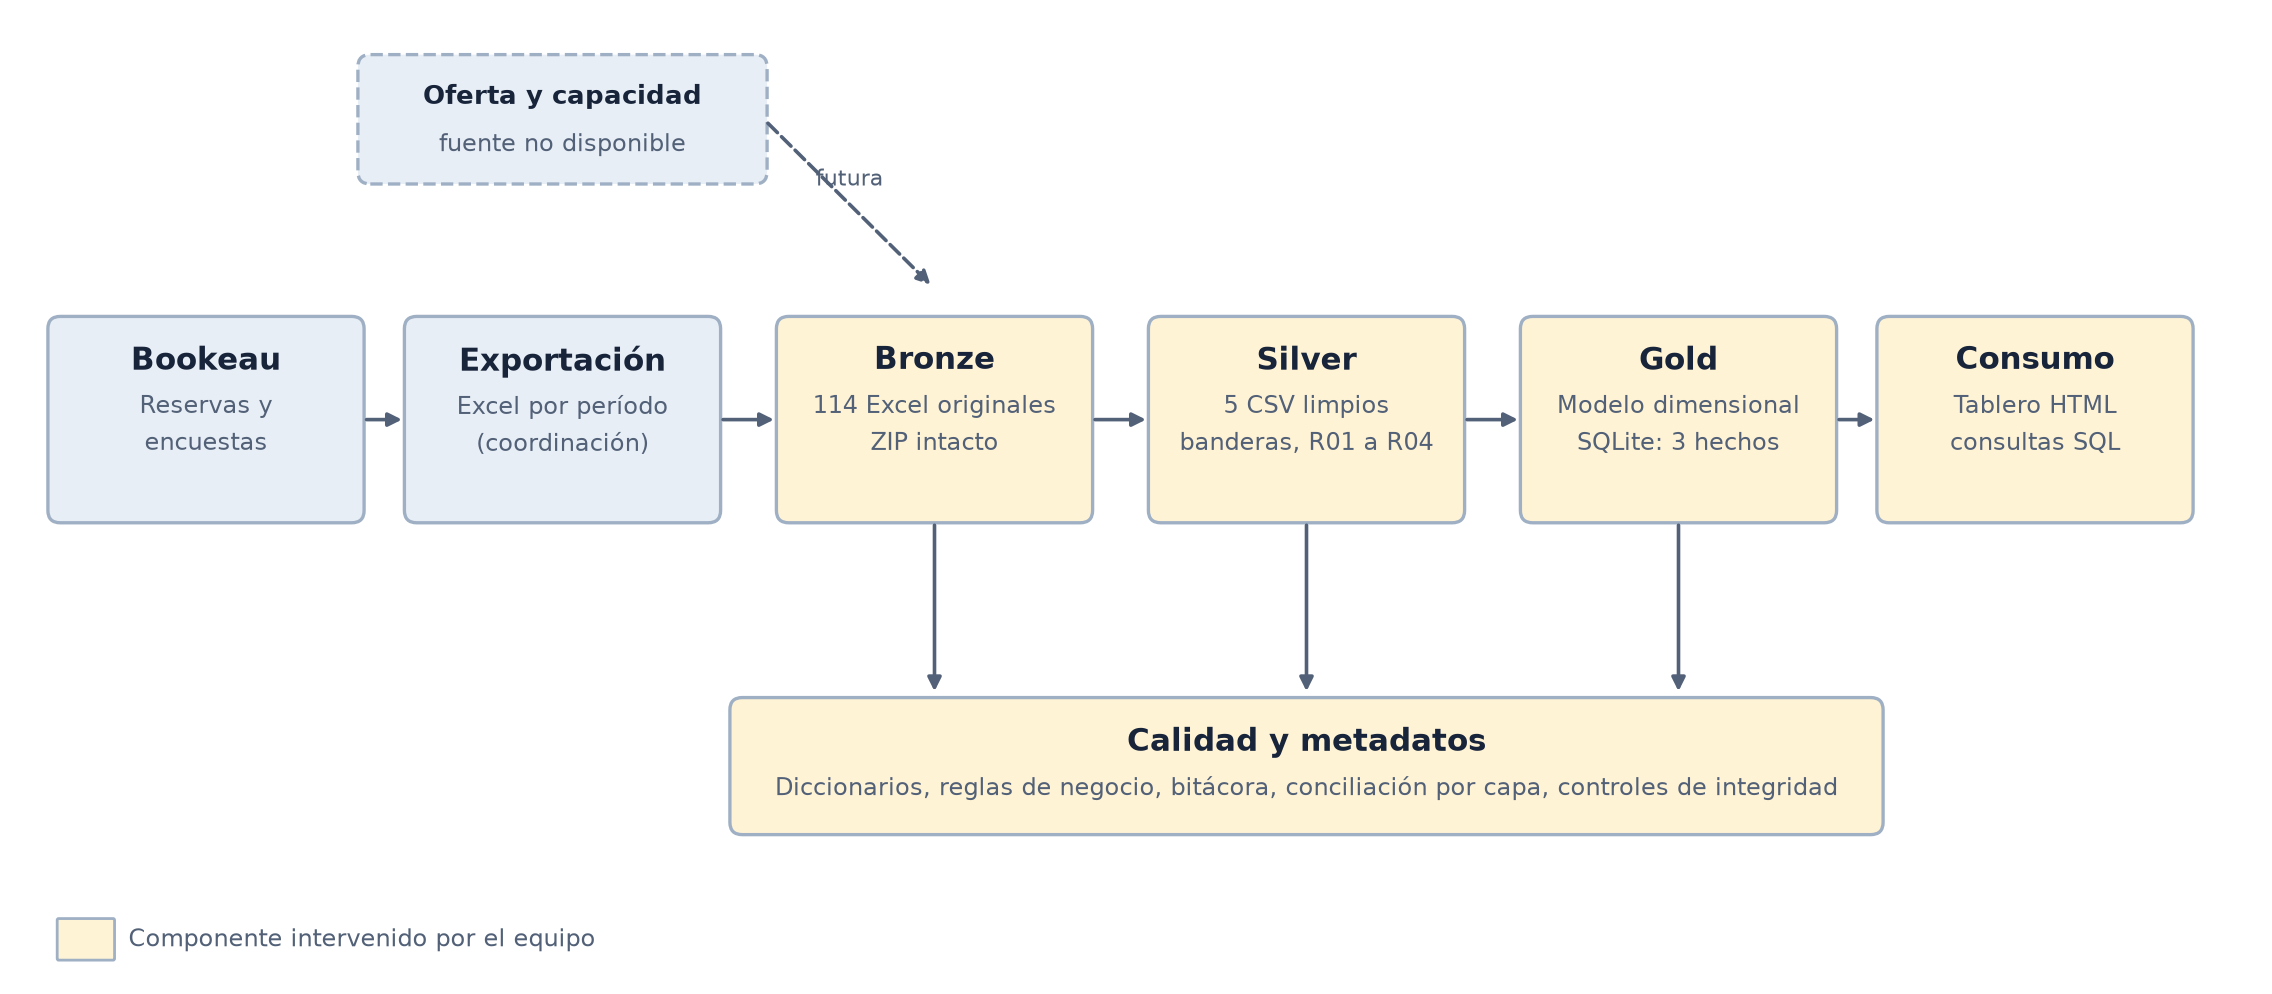
\includegraphics[width=\textwidth,height=0.45\textheight,keepaspectratio]{ecosistema.png}
\caption{Ecosistema de analítica propuesto}
\end{figure}

\begingroup\small\setlength{\tabcolsep}{4pt}\renewcommand{\arraystretch}{1.15}
\begin{longtable}{>{\raggedright\arraybackslash}p{\dimexpr 0.165\textwidth-2\tabcolsep\relax}>{\raggedright\arraybackslash}p{\dimexpr 0.382\textwidth-2\tabcolsep\relax}>{\raggedright\arraybackslash}p{\dimexpr 0.382\textwidth-2\tabcolsep\relax}}
\toprule
\textbf{Componente} & \textbf{Función} & \textbf{Por qué} \\
\midrule
\endhead
Bookeau + exportación & Origen de los datos; la coordinación descarga un Excel por período con todos los servicios y modalidades, y el reporte de horarios por semestre. & Es el único mecanismo de extracción disponible; no hay acceso directo a la base de datos de Bookeau. \\
\textbf{Bronze} & Guarda los archivos originales sin modificar (un ZIP con los 114 Excel de reservas y encuestas y los 30 de horarios). & Permite volver a empezar desde cero y rastrear cualquier cifra hasta la celda de origen. \\
\textbf{Silver} & Un archivo CSV (texto con columnas separadas por comas) por fuente, ya limpio: nombres de columna iguales entre fuentes, fechas en formato estándar (ISO 8601, año-mes-día), tipos de dato explícitos, programa académico normalizado, reglas de negocio aplicadas y \textbf{banderas} (columnas que marcan filas sospechosas). & La limpieza se hace una sola vez y todos los análisis la reutilizan. No se borra ningún registro. \\
\textbf{Gold} & La base de datos final, organizada como \textbf{modelo dimensional} (sección 4): 4 tablas de hechos y 10 de dimensiones, en SQLite, con restricciones de integridad. & Responde los dos análisis con las mismas categorías para ambos y sin contar dos veces un mismo evento. \\
Consumo & Un tablero en HTML (un archivo que se abre en el navegador, sin servidor) y consultas en SQL (el lenguaje estándar para consultar bases de datos). & La coordinación puede abrirlo directamente, sin instalar nada. \\
Calidad y metadatos & Diccionarios (qué significa cada columna), reglas de negocio, bitácora de transformaciones y conciliación entre capas (comparar cuántos registros entran y salen). & Cada decisión queda documentada y se puede verificar. \\
\bottomrule
\end{longtable}
\endgroup


\textbf{Qué se interviene y cómo.} Bronze contiene las 114 hojas originales (carga e inventario). Silver conserva los 146.952 registros de reservas y encuestas y las 1.396 franjas de horarios (limpieza y reglas). Gold conserva las reservas de tutorías (regla R03), excluye las encuestas inválidas (regla R02) y carga la oferta; allí se construyen el modelo y la carga, y las respuestas de texto se guardan con su vínculo a la pregunta y a la encuesta para las siguientes entregas. También se interviene el consumo (tablero) y la capa de calidad.

\textbf{Implementación y migración.} Para esta entrega la implementación es local, con programas en Python, archivos CSV y la base de datos SQLite (un motor de base de datos contenido en un solo archivo). No está conectada a Bookeau ni desplegada en la nube, y no se declara que exista un lakehouse corporativo. Los criterios de diseño no dependen de la plataforma: una migración a un lakehouse administrado en la nube (por ejemplo, con el formato Delta Lake) debe mantener las granularidades, las reglas, las restricciones y la conciliación, sin cambiar el modelo; formatos, catálogo, acceso, orquestación y carga incremental se decidirían según esa plataforma.

\textbf{Oferta y capacidad.} Los horarios aportan la oferta por semestre, día y hora de la categoría Tutor Presencial. No traen la oferta por fecha concreta, servicio ni modalidad, así que no se mide la ocupación de una sesión puntual ni la de categorías sin horarios, y no se publica demanda insatisfecha fuera de las franjas con datos. Los cupos disponibles son la capacidad total de la franja en el semestre, y los reservados son los ya tomados (definición confirmada por la coordinación). Entre 202220 y 202320 la oferta presencial casi no existe porque no hubo tutorías presenciales. Para medir ocupación por sesión harían falta registros de las sesiones ofrecidas por fecha, con capacidad y cambios de disponibilidad; su granularidad sería distinta de la de la franja semanal.

\subsection{Pertinencia del ecosistema}

\begingroup\small\setlength{\tabcolsep}{4pt}\renewcommand{\arraystretch}{1.15}
\begin{longtable}{>{\raggedright\arraybackslash}p{\dimexpr 0.381\textwidth-2\tabcolsep\relax}>{\raggedright\arraybackslash}p{\dimexpr 0.549\textwidth-2\tabcolsep\relax}}
\toprule
\textbf{Criterio de buena práctica} & \textbf{Cómo lo cumple la propuesta} \\
\midrule
\endhead
Separación por capas & Bronze conserva el original, Silver limpia sin borrar y Gold sirve el modelo. Cada capa tiene un solo propósito. \\
Reproducibilidad y trazabilidad & Cada paso es un programa guardado; cada registro de Gold conserva el archivo, la hoja y la fila de Excel de donde vino. \\
Metadatos y calidad en todas las capas & Diccionarios, reglas, bitácora y conciliación acompañan los datos. \\
Proporcionalidad & Con 83.894 reservas, 383.183 respuestas y 1.396 franjas de oferta, un motor local basta. No se propone un orquestador (programa que lanza y vigila los pasos en secuencia) ni un almacén en la nube que el volumen no justifica. \\
Capacidad de evolución & El modelo no depende de la plataforma; la oferta de franjas y el texto son extensiones previstas. \\
\bottomrule
\end{longtable}
\endgroup



\section{Exploración y calidad de datos}

Revisamos los 114 archivos completos, sin tomar muestras. Las estadísticas de esta sección describen todas las reservas recibidas, antes de aplicar la regla R03, y los horarios completos. Las tablas completas están en el Anexo C.

\subsection{Estadísticas descriptivas}

\begingroup\small\setlength{\tabcolsep}{4pt}\renewcommand{\arraystretch}{1.15}
\begin{longtable}{>{\raggedright\arraybackslash}p{\dimexpr 0.435\textwidth-2\tabcolsep\relax}>{\raggedright\arraybackslash}p{\dimexpr 0.495\textwidth-2\tabcolsep\relax}}
\toprule
\textbf{Variable (Reservas)} & \textbf{Resultado} \\
\midrule
\endhead
Rango de inicio programado & 19 de agosto de 2016 a 22 de mayo de 2026, 29 períodos \\
Duración programada & mínimo 20, mediana 50, máximo 120 minutos \\
Estados & 12 etiquetas: Finalizada 38.541 · Cancelada a tiempo 18.147 · En cola 10.215 · No asistió 5.086 · Cola cancelada por reservación 4.603 · Realizada 4.105 · otras 5.865 \\
Servicios (el curso para el que se pide la tutoría) & 11: IP 53.272 · APO 1 (histórico) 21.136 · EDA 6.127 · APO 2 3.922 · otros 2.105 \\
Modalidades (tipo de horario) & 10: Normal 49.472 · Express 25.754 · Normal pico 8.668 · otras 2.668 \\
Cantidad de valores distintos & 9.943 códigos de usuario · 742 prestadores (monitores) · 213 etiquetas de programa académico \\
Hora de inicio más frecuente & 11:00 (13.699), 14:00 (11.253), 09:00 (10.217) \\
\bottomrule
\end{longtable}
\endgroup


\begingroup\footnotesize\setlength{\tabcolsep}{4pt}\renewcommand{\arraystretch}{1.15}
\begin{longtable}{>{\raggedright\arraybackslash}p{\dimexpr 0.275\textwidth-2\tabcolsep\relax}>{\raggedleft\arraybackslash}p{\dimexpr 0.109\textwidth-2\tabcolsep\relax}>{\raggedleft\arraybackslash}p{\dimexpr 0.109\textwidth-2\tabcolsep\relax}>{\raggedleft\arraybackslash}p{\dimexpr 0.109\textwidth-2\tabcolsep\relax}>{\raggedleft\arraybackslash}p{\dimexpr 0.109\textwidth-2\tabcolsep\relax}>{\raggedleft\arraybackslash}p{\dimexpr 0.109\textwidth-2\tabcolsep\relax}>{\raggedleft\arraybackslash}p{\dimexpr 0.109\textwidth-2\tabcolsep\relax}}
\toprule
\textbf{Calificación del tutor (encuestas válidas)} & \textbf{1} & \textbf{2} & \textbf{3} & \textbf{4} & \textbf{5} & \textbf{Sin nota} \\
\midrule
\endhead
Encuestas & 122 & 152 & 648 & 2.031 & 13.218 & 6.803 \\
\% sobre calificadas & 0,8\% & 0,9\% & 4,0\% & 12,6\% & 81,7\% & --- \\
\bottomrule
\end{longtable}
\endgroup


\textbf{Horarios (oferta).} Hay 1.396 franjas en 30 archivos; 142 tienen cupos reservados y disponibles en 0 (franjas sin oferta ni actividad).

\begingroup\small\setlength{\tabcolsep}{4pt}\renewcommand{\arraystretch}{1.15}
\begin{longtable}{>{\raggedright\arraybackslash}p{\dimexpr 0.582\textwidth-2\tabcolsep\relax}>{\raggedleft\arraybackslash}p{\dimexpr 0.164\textwidth-2\tabcolsep\relax}>{\raggedleft\arraybackslash}p{\dimexpr 0.183\textwidth-2\tabcolsep\relax}}
\toprule
\textbf{Medida de los horarios} & \textbf{Total} & \textbf{Máximo por franja} \\
\midrule
\endhead
Asistencias & 27.835 & 76 \\
Cancelaciones & 14.768 & 44 \\
Inasistencias & 3.019 & 14 \\
En lista de espera & 6.719 & 28 \\
Reservaron luego de estar en lista & 3.534 & 35 \\
Cupos reservados & 30.292 & 83 \\
Cupos disponibles & 46.867 & 94 \\
\bottomrule
\end{longtable}
\endgroup


\subsection{Completitud}

La \textbf{completitud} mide los datos faltantes: dónde están, cuántos registros son y qué porcentaje representan.

\begingroup\small\setlength{\tabcolsep}{4pt}\renewcommand{\arraystretch}{1.15}
\begin{longtable}{>{\raggedright\arraybackslash}p{\dimexpr 0.174\textwidth-2\tabcolsep\relax}>{\raggedright\arraybackslash}p{\dimexpr 0.259\textwidth-2\tabcolsep\relax}>{\raggedleft\arraybackslash}p{\dimexpr 0.090\textwidth-2\tabcolsep\relax}>{\raggedleft\arraybackslash}p{\dimexpr 0.056\textwidth-2\tabcolsep\relax}>{\raggedright\arraybackslash}p{\dimexpr 0.351\textwidth-2\tabcolsep\relax}}
\toprule
\textbf{Fuente} & \textbf{Variable} & \textbf{Faltantes} & \textbf{\%} & \textbf{Interpretación} \\
\midrule
\endhead
Todas & Fecha de devolución & 146.952 & 100\% & El campo no se usa; no hay hora real de fin. \textbf{No se puede medir la duración efectiva de la tutoría.} \\
Reservas & Fecha de llegada & 43.422 & 50,2\% & Esperado: las cancelaciones y la cola no tienen llegada. Ver 3.4. \\
Reservas & Prestador del servicio (monitor) & 42.616 & 49,2\% & Esperado: solo las citas atendidas tienen monitor asignado. \\
Reservas & Programa académico & 333 & 0,4\% & Faltante real; se carga como «No informado». \\
Encuesta Express & Calificación del tutor & 1.776 & 26,3\% & La pregunta no existía antes del período 201819. \\
Encuesta Normal & Calificación del tutor & 5.053 & 30,9\% & Igual que la anterior. \\
Encuestas de satisfacción & Comprensión del tema / material del curso & 16.786 & 72--73\% & Preguntas añadidas en períodos recientes. \\
Encuestas de satisfacción & Comentario sobre tutor y tutoría & 5.151 & 19--23\% & Texto opcional. \\
Horarios & Archivos sin franjas & 3 de 30 & 10\% & 202219, 202220 y 202319: no hubo tutorías presenciales. \\
Horarios & Cupos reservados & 288 & 20,6\% & Es 0 en 201620 y 201710 (135 franjas, no registrado); en las otras 153 la franja no tuvo actividad. \\
\bottomrule
\end{longtable}
\endgroup


Los faltantes de las encuestas se explican por \textbf{cambios del formulario en el tiempo}; la cobertura de cada pregunta por período (primer período con valores) está en el Anexo C.5.

\subsection{Unicidad}

La \textbf{unicidad} revisa que no haya registros repetidos, ni completos ni en lo que los identifica.

\begingroup\small\setlength{\tabcolsep}{4pt}\renewcommand{\arraystretch}{1.15}
\begin{longtable}{>{\raggedright\arraybackslash}p{\dimexpr 0.465\textwidth-2\tabcolsep\relax}>{\raggedright\arraybackslash}p{\dimexpr 0.465\textwidth-2\tabcolsep\relax}}
\toprule
\textbf{Comprobación} & \textbf{Resultado} \\
\midrule
\endhead
Filas idénticas en todas las columnas, en cada fuente & 0 \\
ID repetido dentro de cada fuente & 0 (86.562 ID únicos en Reservas) \\
ID + período repetido & 0 \\
Encuestas sin reserva correspondiente & 0 de 60.390 (todas se vinculan por ID y período) \\
Más de una encuesta del mismo tipo por reserva & 0 \\
Franjas repetidas (período, día, hora) en horarios & 0 \\
Repeticiones de significado: variantes de escritura del programa académico & 213 etiquetas $\rightarrow$ 174 tras normalizar mayúsculas, tildes y espacios (Anexo C.11) \\
\bottomrule
\end{longtable}
\endgroup


\subsection{Consistencia}

La \textbf{consistencia} revisa que los datos sean coherentes entre sí y estén escritos de forma uniforme. El detalle por variable y encuesta está en el Anexo C.7, y el cruce entre estados y llegada en el Anexo C.4.

\begingroup\small\setlength{\tabcolsep}{4pt}\renewcommand{\arraystretch}{1.15}
\begin{longtable}{>{\raggedright\arraybackslash}p{\dimexpr 0.318\textwidth-2\tabcolsep\relax}>{\raggedleft\arraybackslash}p{\dimexpr 0.168\textwidth-2\tabcolsep\relax}>{\raggedleft\arraybackslash}p{\dimexpr 0.127\textwidth-2\tabcolsep\relax}>{\raggedright\arraybackslash}p{\dimexpr 0.318\textwidth-2\tabcolsep\relax}}
\toprule
\textbf{Comprobación} & \textbf{Casos} & \textbf{\%} & \textbf{Tratamiento} \\
\midrule
\endhead
Estado cancelado con marca de llegada & 32 & 0,04\% & Se marca con una bandera para revisión \\
Estado Finalizada sin marca de llegada & 8 & 0,01\% & Bandera \\
No asistió con marca de llegada & 9 & 0,18\% de No asistió & Bandera \\
El estado de la reserva difiere entre el archivo de reservas y el de la encuesta & 73 & 0,1\% & Gold usa el valor del archivo de reservas; la diferencia queda guardada \\
El monitor difiere entre reserva y encuesta & 550 & 1,0--1,6\% & Igual que la anterior \\
El programa académico difiere entre reserva y encuesta & 97 & 0,1--0,2\% & Igual que la anterior \\
Encabezado escrito de dos formas («Código servicio» y «Código del servicio») & 4 fuentes & --- & Se unifica el nombre de columna en Silver \\
El grupo de archivo no coincide con la modalidad registrada & 1.609 encuestas & --- & El archivo \emph{Encuesta Normal} contiene 1.461 encuestas de «Normal pico»; se segmenta por la modalidad de la reserva \\
Etiquetas marcadas \texttt{Deprecated} (obsoletas) en el origen & 6 servicios y 5 modalidades & --- & Se conservan como categorías propias, sin unirlas con otras \\
Horarios frente a Reservas (Tutor Presencial): franjas con las cinco medidas iguales & 1.386 de 1.396 & 99,3\% & Las 10 que difieren son de 202619, período que no está en Reservas; se conservan \\
\bottomrule
\end{longtable}
\endgroup


\textbf{Qué confirman los horarios.} Comparados por período, día y hora con Reservas de categoría Tutor Presencial, los cinco conteos de los horarios coinciden exactamente con estas sumas de estados: Asistencias = Finalizada + Realizada + En ejecución; Inasistencias = No asistió; Cancelaciones = todos los estados «Cancelada\ldots{}»; En lista de espera = En cola; y Reservaron luego de estar en lista = Cola cancelada por reservación. Eso aclara el significado de esta última etiqueta, que antes no estaba documentado. La coincidencia es exacta en los 26 períodos que tienen franjas y reservas; los horarios no incluyen otras categorías (entre 202210 y 202410 la mayoría de las tutorías se registró en otras categorías, por lo que los horarios cubren solo una parte de las atenciones de esos semestres).

\subsection{Validez}

La \textbf{validez} revisa que el valor de cada dato tenga sentido en el contexto del problema. Las reglas evaluadas en cada fuente están en el Anexo C.8.

\begingroup\small\setlength{\tabcolsep}{4pt}\renewcommand{\arraystretch}{1.15}
\begin{longtable}{>{\raggedright\arraybackslash}p{\dimexpr 0.607\textwidth-2\tabcolsep\relax}>{\raggedleft\arraybackslash}p{\dimexpr 0.167\textwidth-2\tabcolsep\relax}>{\raggedleft\arraybackslash}p{\dimexpr 0.156\textwidth-2\tabcolsep\relax}}
\toprule
\textbf{Regla} & \textbf{Evaluables} & \textbf{Incumplen} \\
\midrule
\endhead
Fin programado $\geq$ inicio programado & 146.952 & 0 \\
El año del inicio coincide con el año del código de período & 146.952 & 0 \\
Calificación del tutor entre 1 y 5 & 16.309 & 0 \\
Llegada más de 1 hora antes del inicio & 43.140 & 37 \\
Llegada después del fin programado & 43.140 & 45 \\
Citas pasadas que siguen en estado no terminal («En ejecución» o «Reservada») & 508 & 508 \\
Encuestas marcadas «Inválida» por Bookeau & 60.390 & 166 \\
Franjas de horarios de lunes a viernes & 1.396 & 1 (domingo) \\
Medidas de horarios vacías o negativas & 1.396 & 0 \\
Cupos reservados mayores que los cupos disponibles de la franja & 1.396 & 5 (por un cupo en cada una) \\
\bottomrule
\end{longtable}
\endgroup


Las 508 citas que siguen «En ejecución» o «Reservada» después de su fecha nunca se cerraron. La regla R07 las clasifica: «En ejecución» como atendida, y «Reservada» como atendida solo si tiene hora de llegada y prestador, y como no asistió en los demás casos. En las reservas de tutorías son 461: 298 «En ejecución» y 163 «Reservada» (36 con llegada y prestador, 127 sin alguno de los dos).

\subsection{Transformaciones que se derivan del análisis de calidad}

El análisis anterior define qué debe corregirse al pasar los datos de una capa a otra:

\begin{enumerate}[leftmargin=1.5em,itemsep=2pt]
\item Unificar nombres de columna, escribir las fechas en formato ISO 8601 y fijar los tipos de dato, tratando los identificadores como texto.
\item Normalizar la escritura del programa académico en una columna adicional, conservando el original.
\item Horarios: pasar el día a número ISO y la hora a formato de 24 horas, guardar las siete medidas como enteros y conservar archivo, hoja y fila de origen.
\item Aplicar las reglas R01 a R07 (sección 1.3): R01, R06 y R07 se guardan en el estado analítico de la dimensión Estado (\texttt{estado\_\allowbreak{}analitico}), R04 en su grupo de estado (\texttt{grupo\_\allowbreak{}estado}, ver 4.4), R02 y R03 actúan como filtros en la carga a Gold, y R05 define con qué reservas se compara la oferta.
\item Marcar con banderas los casos inconsistentes, sin corregirlos ni borrarlos.
\item No inventar valores: no se rellenan la fecha de devolución, la llegada ni las calificaciones faltantes.
\end{enumerate}


\section{Modelo de datos conceptual}

Para organizar los datos usamos el \textbf{modelo dimensional} de Ralph Kimball, una forma estándar de diseñar bases de datos pensadas para analizar. Se basa en dos tipos de tablas:

\begin{itemize}[leftmargin=1.5em,itemsep=2pt]
\item \textbf{Tabla de hechos:} registra un evento que se quiere contar o medir. Aquí, una reserva o una encuesta respondida.
\item \textbf{Tabla de dimensión:} describe el contexto del evento y sirve para filtrar y agrupar. Aquí, la fecha, el servicio, la modalidad, el estado y el programa.
\end{itemize}

La \textbf{granularidad} (en inglés, \emph{grain}) dice qué representa exactamente una fila de una tabla de hechos. Definirla primero evita contar dos veces. Kimball propone cuatro pasos de diseño: elegir el proceso de negocio, definir la granularidad, identificar las dimensiones e identificar los hechos.

\subsection{Procesos de negocio y granularidad}

\begingroup\small\setlength{\tabcolsep}{4pt}\renewcommand{\arraystretch}{1.15}
\begin{longtable}{>{\raggedright\arraybackslash}p{\dimexpr 0.117\textwidth-2\tabcolsep\relax}>{\raggedright\arraybackslash}p{\dimexpr 0.271\textwidth-2\tabcolsep\relax}>{\raggedright\arraybackslash}p{\dimexpr 0.271\textwidth-2\tabcolsep\relax}>{\raggedright\arraybackslash}p{\dimexpr 0.271\textwidth-2\tabcolsep\relax}}
\toprule
\textbf{Paso} & \textbf{Proceso 1 · Reserva de tutoría} & \textbf{Proceso 2 · Encuesta de la tutoría} & \textbf{Proceso 3 · Oferta semestral} \\
\midrule
\endhead
1. Proceso de negocio & Solicitud y cierre de una cita en Bookeau & Respuesta del estudiante a la encuesta previa o posterior & Resumen por franja de la oferta y de lo ocurrido en ella (horarios) \\
2. Granularidad & \textbf{Un evento de reserva} (identificado por el ID de Bookeau) & \textbf{Una encuesta válida de una reserva}; en el detalle, \textbf{una respuesta no vacía a una pregunta} & \textbf{Una franja de un semestre}: período $\times$ día de la semana $\times$ hora de inicio (categoría Tutor Presencial) \\
3. Dimensiones & Fecha (de inicio, de fin y de llegada), Hora, Período, Servicio, Modalidad, Estado, Programa & Las mismas, compartidas con la reserva, más Tipo de encuesta; el detalle añade Pregunta & Período, Día de la semana, Hora \\
4. Hechos (medidas) & \texttt{evento\_\allowbreak{}reserva} (siempre 1, para poder sumar), \texttt{minutos\_\allowbreak{}programados}, \texttt{es\_\allowbreak{}prioritaria} & \texttt{respuesta\_\allowbreak{}encuesta} (siempre 1), \texttt{calificacion\_\allowbreak{}ayuda\_\allowbreak{}tutor} (1 a 5, puede estar vacía); el detalle tiene \texttt{valor\_\allowbreak{}original} y \texttt{valor\_\allowbreak{}numerico} & \texttt{asistencias}, \texttt{cancelaciones}, \texttt{inasistencias}, \texttt{en\_\allowbreak{}lista\_\allowbreak{}espera}, \texttt{reservaron\_\allowbreak{}luego\_\allowbreak{}de\_\allowbreak{}lista}, \texttt{cupos\_\allowbreak{}reservados}, \texttt{cupos\_\allowbreak{}disponibles} \\
\bottomrule
\end{longtable}
\endgroup


\subsection{Modelos dimensionales propuestos}

Cada figura muestra una tabla de hechos al centro y las dimensiones alrededor. Esta disposición se llama \emph{esquema en estrella}.

\textbf{Modelo 1 · Reservas} (responde al Análisis 1)

\begin{figure}[H]\centering
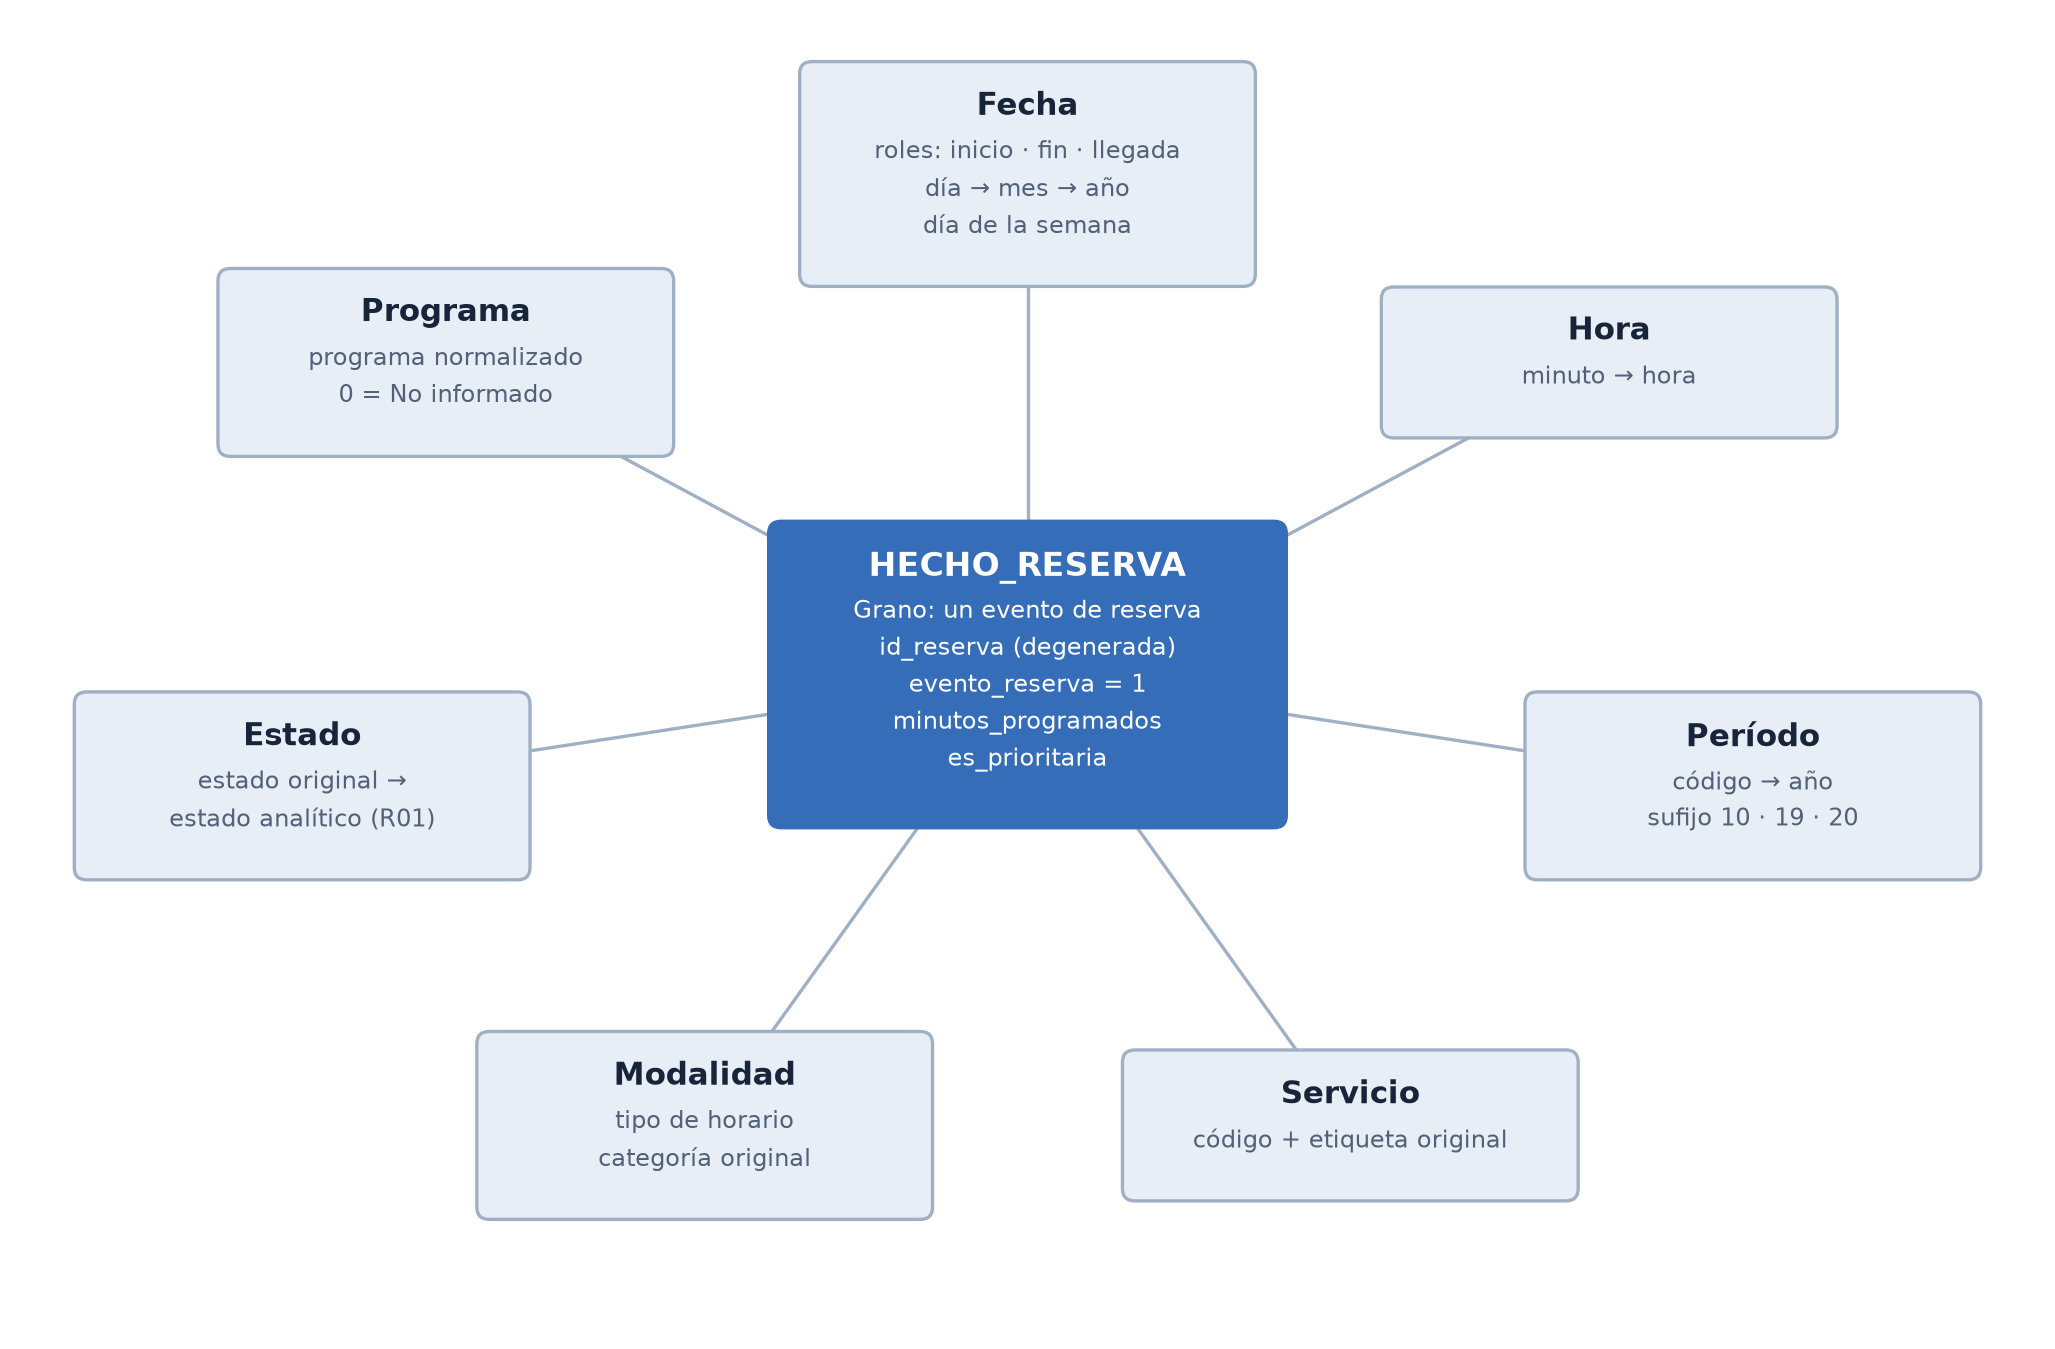
\includegraphics[width=\textwidth,height=0.45\textheight,keepaspectratio]{modelo_reserva.png}
\caption{Modelo dimensional de reservas}
\end{figure}

\textbf{Modelo 2 · Encuestas y respuestas} (responde al Análisis 2 y prepara el análisis de texto)

\begin{figure}[H]\centering
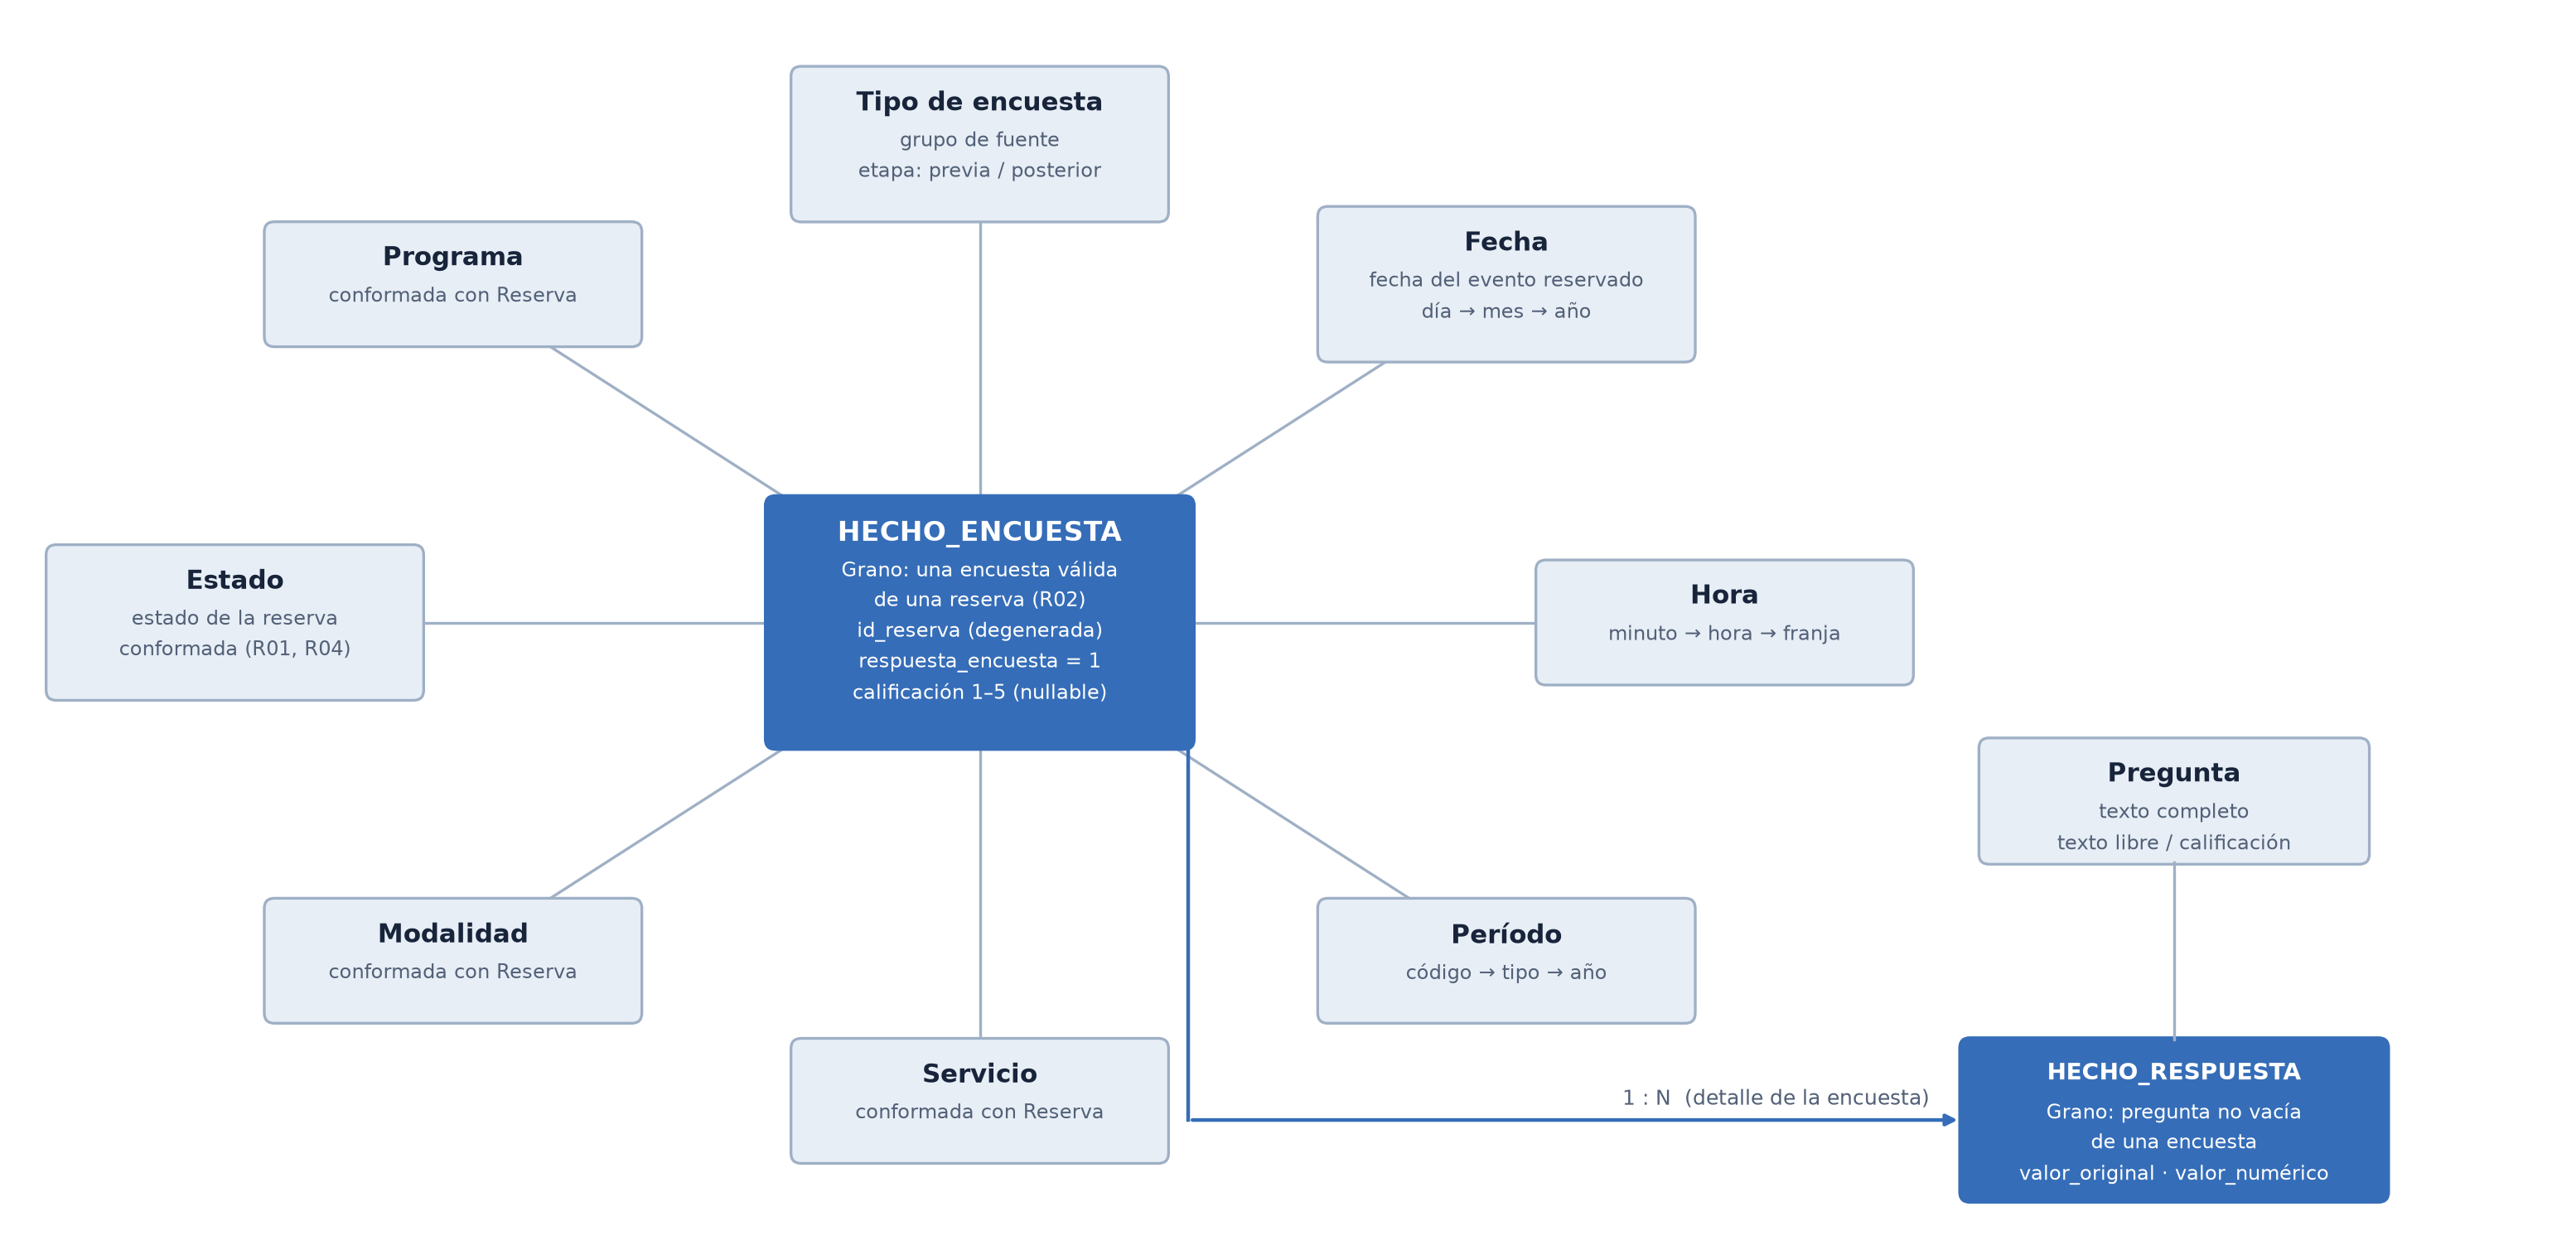
\includegraphics[width=\textwidth,height=0.45\textheight,keepaspectratio]{modelo_encuesta.png}
\caption{Modelo dimensional de encuestas y respuestas}
\end{figure}

\textbf{Modelo 3 · Oferta} (responde a la ocupación y la lista de espera del Análisis 1)

\begin{figure}[H]\centering
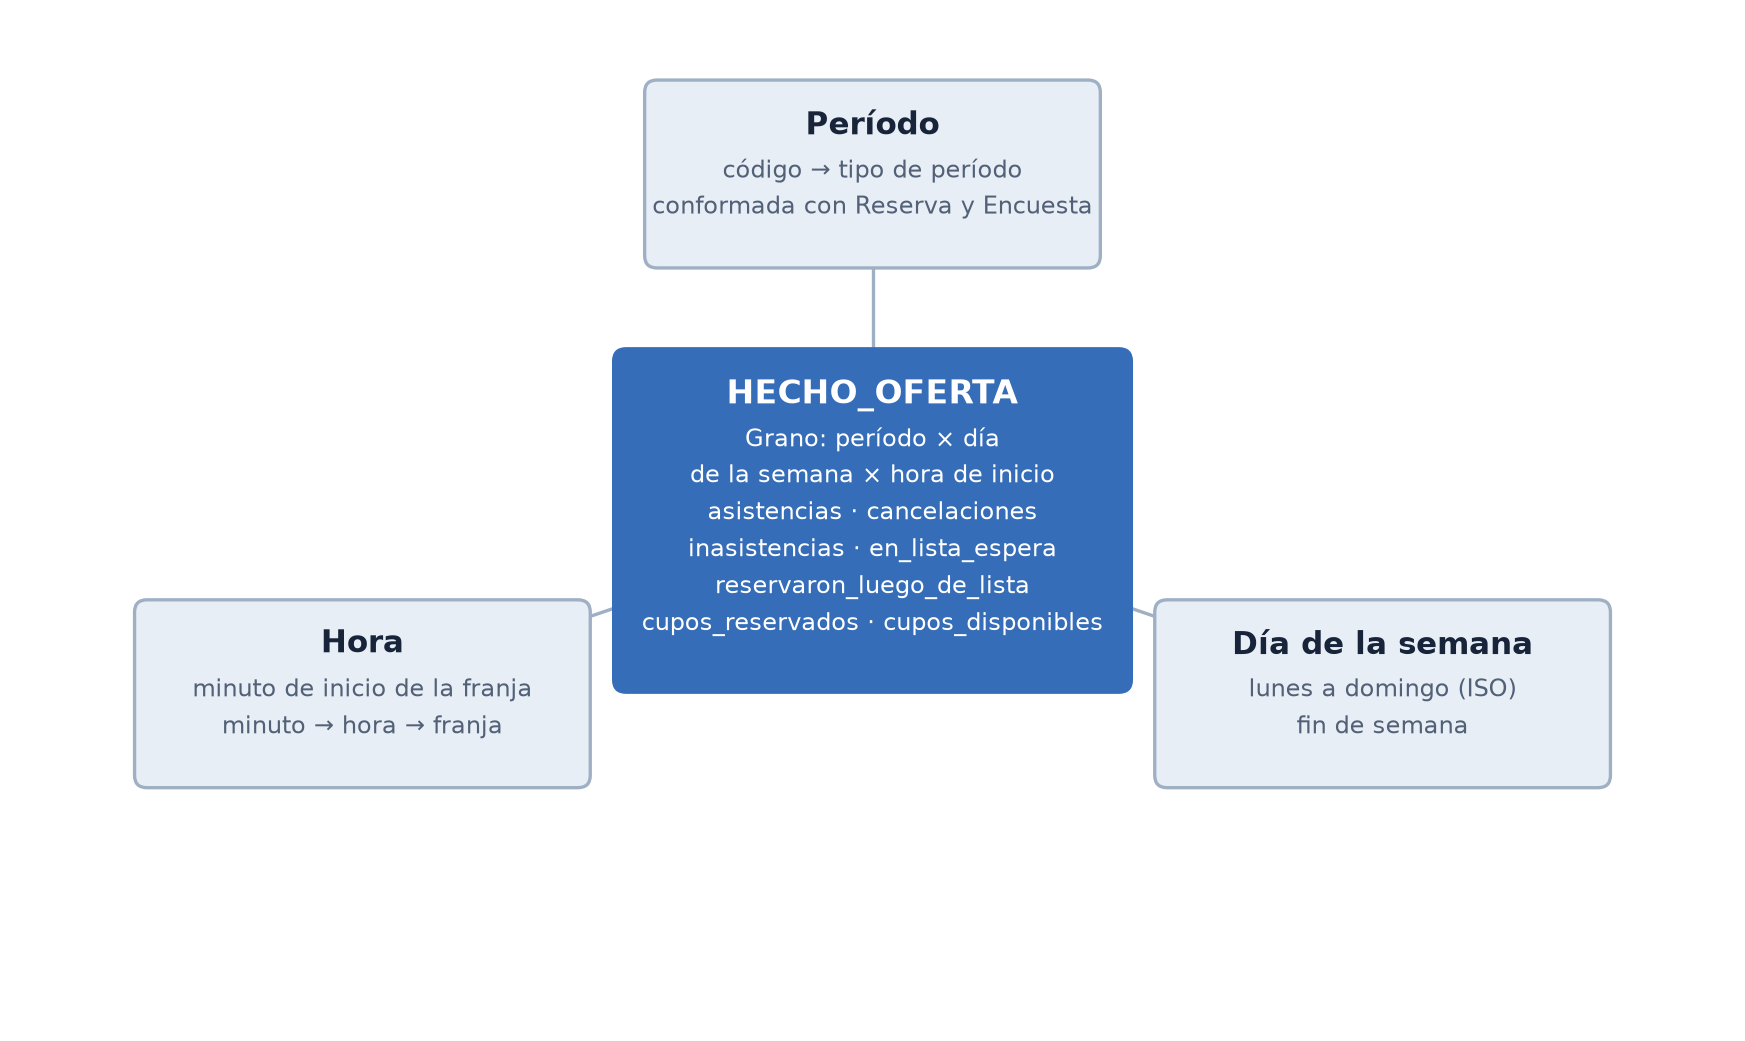
\includegraphics[width=\textwidth,height=0.45\textheight,keepaspectratio]{modelo_oferta.png}
\caption{Modelo dimensional de la oferta}
\end{figure}

\textbf{Dimensiones del modelo y sus jerarquías.} Una \textbf{jerarquía} es una cadena de niveles que permite pasar del detalle al resumen y viceversa (en inglés, \emph{drill-down}). Todas están guardadas en Gold.

\begingroup\small\setlength{\tabcolsep}{4pt}\renewcommand{\arraystretch}{1.15}
\begin{longtable}{>{\raggedright\arraybackslash}p{\dimexpr 0.10\textwidth-2\tabcolsep\relax}>{\raggedright\arraybackslash}p{\dimexpr 0.278\textwidth-2\tabcolsep\relax}>{\raggedright\arraybackslash}p{\dimexpr 0.278\textwidth-2\tabcolsep\relax}>{\raggedright\arraybackslash}p{\dimexpr 0.278\textwidth-2\tabcolsep\relax}}
\toprule
\textbf{Dimensión} & \textbf{Granularidad y atributos} & \textbf{Jerarquía} & \textbf{Motivo} \\
\midrule
\endhead
Fecha & Un día del calendario completo, con tres roles (inicio, fin, llegada); \texttt{nombre\_\allowbreak{}dia}, \texttt{nombre\_\allowbreak{}mes}, \texttt{dia\_\allowbreak{}semana\_\allowbreak{}iso}, \texttt{es\_\allowbreak{}fin\_\allowbreak{}de\_\allowbreak{}semana} & día $\rightarrow$ mes $\rightarrow$ año & Permite series y mostrar fechas sin eventos \\
Período & Código original, año del código y terminación sin reinterpretar & código $\rightarrow$ tipo de período (Semestre 1 = terminación 10, Semestre 2 = 20, Intersemestral = 19) & Separa el período académico exportado de la fecha del calendario; es la dimensión común de reservas, encuestas y oferta \\
Día de la semana & Siete miembros: número ISO, nombre e indicador de fin de semana & Sin jerarquía & La oferta se resume por día de la semana y hora, no por fecha \\
Hora & Un minuto del día (1.440 miembros); \texttt{etiqueta} (HH:MM) & minuto $\rightarrow$ hora $\rightarrow$ franja (Madrugada, Mañana, Tarde, Noche) & Segmenta el inicio programado sin confundirlo con los segundos de la llegada \\
Servicio & Código y etiqueta original & Sin jerarquía (lista plana) & Conserva los catálogos históricos sin fusionar los \texttt{Deprecated} \\
Modalidad & Tipo de horario y categoría originales & Sin jerarquía & Evita confundir la modalidad con el recurso, y los grupos de archivo con modalidades \\
Estado & Etiqueta original, estado analítico (R01, R06 y R07) y grupo (R04); «Reservada» tiene dos miembros, uno por cada resultado de R07 & estado original (12) $\rightarrow$ estado analítico (5) $\rightarrow$ grupo (5) & Conserva la evidencia y permite contar atenciones sin perder el detalle \\
Programa & Etiqueta normalizada; miembro 0 «No informado» & Sin jerarquía & Agrupa variantes de escritura y mantiene explícitos los faltantes. Son etiquetas registradas, no el programa oficial certificado \\
Tipo de encuesta & Grupo de fuente y etapa (previa o posterior) & Sin jerarquía & Define el proceso de encuesta; por sí solo no identifica la modalidad real \\
Pregunta & Texto completo, columna de origen y marcas de texto libre y de calificación & Sin jerarquía & Admite preguntas largas sin un hecho distinto por pregunta \\
\bottomrule
\end{longtable}
\endgroup


Los atributos de segmentación de la encuesta se toman de la reserva vinculada, como referencia de trabajo acordada; las diferencias del registro de la encuesta permanecen en Silver y en la auditoría de Gold. El hecho de encuesta incluye las etapas previa y posterior: la satisfacción filtra la posterior y no se mezcla con las respuestas previas. Las fechas de la encuesta describen la reserva asociada, no el momento en que se contestó.

\subsection{Matriz de bus}

La \textbf{matriz de bus} indica qué dimensiones usa cada tabla de hechos. Una dimensión que usan varias tablas se llama \emph{conformada}: significa lo mismo en todas, y por eso un filtro del tablero sirve para varios análisis.

\begingroup\small\setlength{\tabcolsep}{4pt}\renewcommand{\arraystretch}{1.15}
\begin{longtable}{>{\raggedright\arraybackslash}p{\dimexpr 0.225\textwidth-2\tabcolsep\relax}>{\centering\arraybackslash}p{\dimexpr 0.241\textwidth-2\tabcolsep\relax}>{\centering\arraybackslash}p{\dimexpr 0.225\textwidth-2\tabcolsep\relax}>{\centering\arraybackslash}p{\dimexpr 0.139\textwidth-2\tabcolsep\relax}>{\centering\arraybackslash}p{\dimexpr 0.100\textwidth-2\tabcolsep\relax}}
\toprule
\textbf{Dimensión} & \textbf{Reserva} & \textbf{Encuesta} & \textbf{Respuesta} & \textbf{Oferta} \\
\midrule
\endhead
Fecha (tres roles) & $\checkmark$ inicio · fin · llegada & $\checkmark$ inicio de la reserva & vía encuesta &  \\
Período & $\checkmark$ & $\checkmark$ & vía encuesta & $\checkmark$ \\
Día de la semana &  &  &  & $\checkmark$ \\
Hora & $\checkmark$ & $\checkmark$ & vía encuesta & $\checkmark$ \\
Servicio & $\checkmark$ & $\checkmark$ & vía encuesta &  \\
Modalidad & $\checkmark$ & $\checkmark$ & vía encuesta &  \\
Estado (de la reserva) & $\checkmark$ & $\checkmark$ & vía encuesta &  \\
Programa & $\checkmark$ & $\checkmark$ & vía encuesta &  \\
Tipo de encuesta &  & $\checkmark$ & vía encuesta &  \\
Pregunta &  &  & $\checkmark$ &  \\
\bottomrule
\end{longtable}
\endgroup


La oferta se cruza con las reservas por las dimensiones que comparten: período y hora, y el día de la semana (que se obtiene de la fecha de inicio de la reserva).

\textbf{Medidas y aditividad.} Los conteos unitarios son aditivos dentro de su granularidad. Los minutos programados son aditivos como tiempo reservado, pero pueden superponerse entre recursos o usuarios y no equivalen a horas trabajadas ni a ocupación. La calificación no se suma: se calcula su media y mediana con las respuestas no vacías, mostrando el tamaño del grupo. Los porcentajes se recalculan a partir del numerador y el denominador, nunca se suman ni se promedian sin ponderar. Para comparar hechos se agrega primero por las dimensiones compartidas, sin unir filas de preguntas a reservas, para evitar multiplicar conteos. Los cupos y la lista de espera son aditivos entre franjas de un mismo período, pero un mismo estudiante puede esperar en varias franjas; la ocupación y la conversión de la cola se recalculan como cociente de sumas.

\subsection{Decisiones de diseño y su justificación}

\begingroup\small\setlength{\tabcolsep}{4pt}\renewcommand{\arraystretch}{1.15}
\begin{longtable}{>{\raggedright\arraybackslash}p{\dimexpr 0.465\textwidth-2\tabcolsep\relax}>{\raggedright\arraybackslash}p{\dimexpr 0.465\textwidth-2\tabcolsep\relax}}
\toprule
\textbf{Decisión} & \textbf{Justificación} \\
\midrule
\endhead
\textbf{Tres procesos, cuatro tablas de hechos} & Reserva, encuesta y oferta tienen granularidades distintas. Mezclarlas en una sola tabla repetiría la reserva por cada encuesta, y contar filas daría más eventos de los reales (146.952 en vez de 86.562). La oferta se registra por franja de un semestre, no por reserva. \\
\texttt{hecho\_\allowbreak{}reserva} es una \textbf{tabla de hechos sin medidas numéricas propias} (\emph{factless}) & El proceso solo registra que un evento ocurrió; las preguntas se responden contando filas por estado. La columna \texttt{evento\_\allowbreak{}reserva = 1} hace explícita esa cuenta. \\
\texttt{hecho\_\allowbreak{}respuesta} es un \textbf{detalle con dimensión Pregunta} & Hay 22 preguntas que cambian según el período y el grupo. Una columna por pregunta dejaría la tabla llena de vacíos y obligaría a cambiar la estructura con cada formulario nuevo. Con la dimensión Pregunta, un formulario nuevo solo agrega filas. Los textos libres quedan listos para la Entrega 2. \\
\texttt{id\_\allowbreak{}reserva} como \textbf{dimensión degenerada} & Es un identificador que no tiene atributos propios, así que no necesita tabla de dimensión: se guarda en la tabla de hechos. Permite rastrear y vincular reserva y encuesta. En Gold se protege con una clave foránea (ver 4.5). \\
\textbf{Fecha con roles} (inicio, fin, llegada) & Una sola tabla de calendario sirve tres significados. \\
\textbf{Dimensiones conformadas} entre reserva y encuesta & La encuesta toma servicio, modalidad, estado y programa de su reserva, así que un mismo filtro del tablero se aplica a ambos análisis. \\
\textbf{Modalidad} = tipo de horario + categoría & Es una dimensión pequeña (15 combinaciones tras la regla R03) que evita tener dos dimensiones casi vacías. \\
\textbf{Estado} con jerarquía: original $\rightarrow$ analítico $\rightarrow$ grupo & Las reglas de negocio viven en la dimensión, no en cada consulta: \texttt{estado\_\allowbreak{}analitico} aplica las reglas R01, R06 y R07 y \texttt{grupo\_\allowbreak{}estado} aplica la regla R04 (Atendida, No asistió, Cola, Cola a reserva, Cancelada). Si la coordinación cambia una regla, se modifica una fila de la dimensión y ninguna consulta. \\
\textbf{Manejo de cambios en el tiempo (SCD)} & Servicio, Modalidad y Estado son tipo 0; Programa es tipo 1. La justificación completa está en 4.6. \\
Oferta por franja semanal, no por sesión & Los horarios resumen la oferta por franja de un semestre; el modelo no inventa la oferta por fecha concreta. \\
\textbf{Período como dimensión propia} & La oferta se registra por semestre y no tiene fecha: para cruzarla con reservas y encuestas necesita una dimensión de período compartida. Repetir el período como atributo de Fecha lo duplicaría. \\
\textbf{Día de la semana como dimensión propia} & La oferta se resume por día de la semana y hora, no por fecha. \\
\textbf{Capacidad igual a los cupos disponibles} & Los cupos disponibles ya son la capacidad total de la franja en el semestre (confirmado por la coordinación), por lo que no se suman a los reservados. La ocupación se calcula en la consulta y no se guarda. \\
Sin dimensión de personas & Los análisis no la necesitan, y así se evita exponer datos personales de estudiantes y monitores. \\
\bottomrule
\end{longtable}
\endgroup


\subsection{Criterios de calidad del modelo}

Para decidir si el modelo es bueno usamos los siguientes criterios, cada uno con una forma concreta de comprobarlo.

\begingroup\small\setlength{\tabcolsep}{4pt}\renewcommand{\arraystretch}{1.15}
\begin{longtable}{>{\raggedright\arraybackslash}p{\dimexpr 0.319\textwidth-2\tabcolsep\relax}>{\raggedright\arraybackslash}p{\dimexpr 0.319\textwidth-2\tabcolsep\relax}>{\raggedright\arraybackslash}p{\dimexpr 0.293\textwidth-2\tabcolsep\relax}}
\toprule
\textbf{Criterio} & \textbf{Cómo se verifica} & \textbf{Resultado} \\
\midrule
\endhead
\textbf{Granularidad declarada y única} & \textbf{Clave primaria} (PK, el identificador único de cada fila) en cada hecho, y restricciones de unicidad \texttt{UNIQUE(id\_\allowbreak{}reserva, tipo\_\allowbreak{}encuesta)} y (período, día, hora) en la oferta & 0 violaciones \\
\textbf{Integridad referencial} (ninguna fila apunta a algo que no existe) & \textbf{Claves foráneas} (FK, referencias de una tabla a otra) activas en SQLite y la verificación \texttt{PRAGMA foreign\_\allowbreak{}key\_\allowbreak{}check} & 0 filas huérfanas \\
\textbf{Conservación} (no se pierde ni se inventa nada) & Los registros de Silver son iguales a los de Gold más las exclusiones documentadas, por fuente & 83.894 reservas de Gold + 2.668 excluidas por R03 = 86.562; las encuestas y las 1.396 franjas concilian (sección 5.4) \\
\textbf{Suma correcta de medidas} & Reglas de aditividad de la sección 4.3: conteos por fila, calificaciones solo promediadas y porcentajes recalculados & Revisado en las consultas del tablero \\
\textbf{Sin vacíos en las claves de dimensión} & Categoría «No informado» (clave 0) en Programa & 163 reservas apuntan a la clave 0 \\
\textbf{Valores permitidos en los atributos de agrupación} & Restricciones \texttt{CHECK} (la base rechaza valores fuera de una lista o rango) sobre \texttt{grupo\_\allowbreak{}estado}, \texttt{franja} y \texttt{es\_\allowbreak{}fin\_\allowbreak{}de\_\allowbreak{}semana} & 0 violaciones \\
\textbf{Aptitud para las preguntas} & Cada pregunta de 1.4 y 1.5 se responde con una agrupación (\texttt{GROUP BY}) sobre una sola tabla de hechos y sus dimensiones & Ver las consultas en el Anexo C.13 \\
\textbf{Trazabilidad} & Cada hecho conserva el archivo, la hoja y la fila de Excel de origen & 100\% de las filas \\
\textbf{Reconciliación entre fuentes} & Horarios frente a Reservas (Tutor Presencial), por período, día y hora & 1.386 de 1.396 franjas coinciden en las cinco medidas; las otras 10, de 202619, no existen en Reservas \\
\bottomrule
\end{longtable}
\endgroup


Estos criterios sirven para comprobar la estructura y la conservación de los datos en esta entrega, pero no sustituyen la confirmación de formularios históricos, de la identidad de los participantes ni de los estados operativos desconocidos. Bastan para esta entrega porque cubren los tres fallos típicos de un modelo dimensional: granularidad mal definida (se cuentan eventos de más), integridad rota (filas que desaparecen al cruzar tablas) y medidas mal agregadas (promedios de promedios). Cada criterio se verifica automáticamente en cada carga. La validez de los significados de los estados depende de reglas de negocio, y las que faltan se listan en 5.5.

\subsection{Historia de atributos (SCD)}

Los atributos de una dimensión pueden cambiar con el tiempo (por ejemplo, un servicio cambia de nombre). Las \textbf{dimensiones de cambio lento} (SCD, por \emph{slowly changing dimensions}) son las estrategias para decidir qué se hace con ese cambio:

\begin{itemize}[leftmargin=1.5em,itemsep=2pt]
\item \textbf{Tipo 0:} el valor no cambia nunca; se guarda tal como se registró.
\item \textbf{Tipo 1:} se sobrescribe el valor viejo; no queda historia.
\item \textbf{Tipo 2:} se agrega una fila nueva con fechas de vigencia; se conserva la historia completa.
\end{itemize}

\begingroup\small\setlength{\tabcolsep}{4pt}\renewcommand{\arraystretch}{1.15}
\begin{longtable}{>{\raggedright\arraybackslash}p{\dimexpr 0.199\textwidth-2\tabcolsep\relax}>{\raggedright\arraybackslash}p{\dimexpr 0.271\textwidth-2\tabcolsep\relax}>{\raggedright\arraybackslash}p{\dimexpr 0.460\textwidth-2\tabcolsep\relax}}
\toprule
\textbf{Dimensión} & \textbf{Tipo} & \textbf{Justificación frente al análisis} \\
\midrule
\endhead
Servicio & \textbf{Tipo 0} & El Análisis 2 compara períodos y la transición de APO a IP es un hallazgo en sí. Sobrescribir o unir etiquetas ocultaría ese cambio. Las etiquetas \texttt{Deprecated} se conservan como categorías propias. \\
Modalidad & \textbf{Tipo 0} & Igual que Servicio: Normal, Express y Normal pico son políticas distintas y su historia se lee en cada reserva. \\
Estado & \textbf{Tipo 0} (con reglas versionadas) & El estado de una reserva es un hecho ocurrido, no un atributo que cambie. Las reglas R01, R04, R06 y R07 viven como atributos de la dimensión; si cambian, se documenta la versión y se vuelve a cargar. \\
Programa & \textbf{Tipo 1} & Las variantes de escritura son errores, no cambios reales (213 etiquetas pasan a 174 al normalizar). Corregir sobrescribiendo es lo correcto. \\
Período, Fecha, Día de la semana, Hora & Estáticas & Son calendarios; no cambian. \\
Persona (no modelada) & Tipo 2, si se agregara & Solo un cambio real de programa del estudiante justificaría una fila nueva con vigencia. Hoy no se modela porque ningún análisis lo requiere. \\
\bottomrule
\end{longtable}
\endgroup


Se elige tipo 0 en lugar de tipo 2 porque la fuente no registra cuándo cambió un catálogo: no hay fechas de vigencia que sustenten un tipo 2. Como cada reserva ya trae la etiqueta vigente al momento del evento, el tipo 0 conserva la historia sin inventarla. Si la coordinación exportara una tabla de equivalencias con fechas (ver 5.5), Servicio y Modalidad pasarían a tipo 2.

\subsection{Diseño del repositorio}

El \textbf{repositorio} es el lugar y la forma en que se guardan los datos de Gold. Se compararon cuatro alternativas con los criterios de la primera columna. La evaluación (Alta, Media, Baja) es cualitativa y se basa en el volumen y el uso reales: 83.894 reservas, 60.024 encuestas, 383.183 respuestas y 1.396 franjas de oferta, consultadas por una coordinación sin equipo técnico.

\begin{itemize}[leftmargin=1.5em,itemsep=2pt]
\item \textbf{Relacional (SQLite, esquema en estrella):} tablas con filas y columnas, relacionadas por claves, consultadas con SQL.
\item \textbf{Columnar (Parquet y DuckDB):} guarda cada columna por separado, lo que acelera los cálculos sobre muchas filas. Parquet es el formato de archivo y DuckDB el motor de consulta.
\item \textbf{Tabla ancha desnormalizada (CSV):} un solo archivo grande donde cada fila repite todos los atributos de contexto.
\item \textbf{Documental (JSON):} cada registro es un documento con campos anidados.
\end{itemize}

\begingroup\small\setlength{\tabcolsep}{4pt}\renewcommand{\arraystretch}{1.15}
\begin{longtable}{>{\raggedright\arraybackslash}p{\dimexpr 0.212\textwidth-2\tabcolsep\relax}>{\raggedright\arraybackslash}p{\dimexpr 0.212\textwidth-2\tabcolsep\relax}>{\raggedright\arraybackslash}p{\dimexpr 0.180\textwidth-2\tabcolsep\relax}>{\raggedright\arraybackslash}p{\dimexpr 0.177\textwidth-2\tabcolsep\relax}>{\raggedright\arraybackslash}p{\dimexpr 0.150\textwidth-2\tabcolsep\relax}}
\toprule
\textbf{Criterio} & \textbf{Relacional (SQLite, en estrella)} & \textbf{Columnar (Parquet y DuckDB)} & \textbf{Tabla ancha (CSV)} & \textbf{Documental (JSON)} \\
\midrule
\endhead
Rendimiento analítico con este volumen & Alta: con índices, cientos de miles de filas se agrupan sin problema & Alta: lectura por columna, la mejor a gran escala & Media: hay que recorrer todo el archivo & Baja: agregar exige recorrer documentos \\
Escalabilidad & Media: un solo archivo y un solo escritor a la vez & Alta: crece por archivos y particiones & Baja & Media \\
Integridad (PK, FK, CHECK) & Alta: se declara y se verifica al cargar & Baja: sin restricciones declarativas & Baja & Baja \\
Facilidad de consulta & Alta: SQL estándar y cruces entre dimensiones compartidas & Alta: SQL, pero con herramientas menos conocidas & Media: sin dimensiones, los atributos se repiten & Baja \\
Almacenamiento & Media: guarda filas completas & Alta: comprime por columna & Baja: repite atributos en cada fila & Baja \\
Compatibilidad con herramientas de BI (software de tableros) & Alta: se conecta con las herramientas habituales & Media: requiere conector o motor & Media: se importa, pero sin modelo & Baja \\
Costo y operación & Alta: sin servidor ni licencia & Alta: sin servidor & Alta & Media \\
Soporte del modelo dimensional & Alta: un hecho por tabla y dimensiones compartidas & Alta: igual, con tablas en archivos & Baja: no distingue hechos de dimensiones & Baja \\
\bottomrule
\end{longtable}
\endgroup


\textbf{Recomendación.} Para esta entrega, \textbf{relacional con esquema en estrella en SQLite}. Es el único con integridad referencial declarativa, que es el criterio central de calidad del modelo (4.5), y con este volumen su rendimiento sobra. Además, un archivo único se entrega sin infraestructura.

\textbf{Cuándo cambiar.} Si el volumen crece unas cien veces (por ejemplo, al incorporar la oferta de franjas por hora) o si se conecta una herramienta de BI con varios usuarios, conviene migrar a almacenamiento columnar (Parquet con DuckDB, o un almacén administrado). El modelo dimensional no cambia, solo el motor.


\section{Transformación Silver $\rightarrow$ Gold}

Esta sección describe el proceso que convierte los datos limpios de Silver en el modelo dimensional de Gold (sección 4).

\subsection{Entradas y reglas de la transformación}

Se leen los seis archivos CSV de Silver (reservas, cuatro encuestas y horarios), producto de la limpieza descrita en el Anexo C.11 (nombres comunes, fechas ISO, identificadores como texto, programa normalizado, banderas y trazabilidad). De las reservas solo entran las de tutorías (regla R03) y de las encuestas solo las incluidas por la regla R02; un indicador de validez desconocido requiere revisión y se concilia aparte. Las reglas R01, R06 y R07 llegan a \texttt{dim\_\allowbreak{}estado} como estado analítico, junto con el estado original. No se infiere encuesta completa ni duración efectiva. Los servicios y modalidades históricos se mantienen separados, y la segmentación de la encuesta usa la reserva vinculada, sin afirmar que se reconstruyó la verdad histórica.

\subsection{Diseño del proceso}

\begingroup\small\setlength{\tabcolsep}{4pt}\renewcommand{\arraystretch}{1.15}
\begin{longtable}{>{\raggedleft\arraybackslash}p{\dimexpr 0.055\textwidth-2\tabcolsep\relax}>{\raggedright\arraybackslash}p{\dimexpr 0.187\textwidth-2\tabcolsep\relax}>{\raggedright\arraybackslash}p{\dimexpr 0.344\textwidth-2\tabcolsep\relax}>{\raggedright\arraybackslash}p{\dimexpr 0.344\textwidth-2\tabcolsep\relax}}
\toprule
\textbf{Paso} & \textbf{Entrada (Silver)} & \textbf{Acción} & \textbf{Salida (Gold)} \\
\midrule
\endhead
1 & 6 archivos CSV & Validar que el ID sea único, que cada encuesta se vincule a una reserva y a un período, y que no haya franjas repetidas en horarios & --- (el proceso falla si no se cumple) \\
2 & Fechas de todas las fuentes & Crear un calendario continuo, los 1.440 minutos del día y los 7 días de la semana & \texttt{dim\_\allowbreak{}fecha}, \texttt{dim\_\allowbreak{}hora}, \texttt{dim\_\allowbreak{}dia\_\allowbreak{}semana} \\
3 & Reservas y horarios & Extraer las listas de valores distintos (los períodos de reservas y de horarios incluidos), sin equivalencias inventadas, y calcular los atributos de jerarquía (tipo de período, grupo de estado, franja, nombres de día y mes) & \texttt{dim\_\allowbreak{}periodo}, \texttt{dim\_\allowbreak{}servicio}, \texttt{dim\_\allowbreak{}modalidad}, \texttt{dim\_\allowbreak{}estado}, \texttt{dim\_\allowbreak{}programa} \\
4 & Encabezados de las encuestas & Identificar el tipo y la etapa de cada encuesta y el texto completo de cada pregunta & \texttt{dim\_\allowbreak{}tipo\_\allowbreak{}encuesta}, \texttt{dim\_\allowbreak{}pregunta} \\
5 & Archivo de reservas & Cargar las reservas de tutorías (regla R03), con claves sustitutas (números internos que identifican cada fila de una dimensión) y trazabilidad al origen & \texttt{hecho\_\allowbreak{}reserva} \\
6 & 4 archivos CSV de encuestas & Cargar solo las encuestas incluidas por la regla R02 cuya reserva está en Gold; las claves de segmentación se toman de su reserva & \texttt{hecho\_\allowbreak{}encuesta} \\
7 & 4 archivos CSV de encuestas & Generar una fila por cada pregunta contestada & \texttt{hecho\_\allowbreak{}respuesta} \\
8 & Horarios & Cargar una fila por franja, con las claves de período, día de la semana y hora de inicio & \texttt{hecho\_\allowbreak{}oferta} \\
9 & Base de datos temporal & Aplicar restricciones (PK, FK, CHECK), conciliar y publicar & Base de datos SQLite y archivos CSV de Gold \\
\bottomrule
\end{longtable}
\endgroup


No se exige igualdad entre el número de respuestas y el de encuestas porque sus granularidades son distintas. La carga reconstruye todo en una base de datos temporal y solo reemplaza la versión publicada si pasan todos los controles.

\subsection{Decisiones importantes}

\begingroup\small\setlength{\tabcolsep}{4pt}\renewcommand{\arraystretch}{1.15}
\begin{longtable}{>{\raggedright\arraybackslash}p{\dimexpr 0.310\textwidth-2\tabcolsep\relax}>{\raggedright\arraybackslash}p{\dimexpr 0.310\textwidth-2\tabcolsep\relax}>{\raggedright\arraybackslash}p{\dimexpr 0.310\textwidth-2\tabcolsep\relax}}
\toprule
\textbf{Decisión} & \textbf{Alternativa descartada} & \textbf{Motivo} \\
\midrule
\endhead
Todas las reservas de tutorías pasan a Gold, incluidas cola y cancelaciones & Cargar solo las atendidas & El Análisis 1 necesita los estados no atendidos para calcular inasistencia y cola. \\
Las encuestas «Inválida» no pasan a Gold (regla R02) & Cargarlas con un indicador & Ningún análisis las usa. Siguen en Silver para auditoría. \\
La encuesta hereda servicio, modalidad, estado y programa de la reserva & Usar los atributos de la propia encuesta & Garantiza dimensiones compartidas; las diferencias (0,1\% a 1,6\%) se guardan en el campo \texttt{diferencias\_\allowbreak{}con\_\allowbreak{}reserva\_\allowbreak{}json}. \\
Las respuestas vacías no generan fila & Fila con valor vacío & Así la completitud de cada pregunta se calcula exacta: respuestas / encuestas. \\
Solo la calificación de 1 a 5 recibe valor numérico & Convertir las escalas de acuerdo («totalmente de acuerdo»\ldots{}) a números & Esas escalas cambian entre formularios; convertirlas inventaría una métrica. \\
Etiquetas \texttt{Deprecated} sin unir con otras & Unir APO 1 con IP & No hay un catálogo oficial de equivalencias; unirlas mezclaría cursos distintos. \\
«Cola cancelada por reservación» en un grupo propio (\texttt{Cola a reserva}) & Sumarla a «En cola» & Los horarios confirman que son solicitudes que terminaron en una reserva; contarlas como cola exageraría la demanda sin atender. \\
Todos los estados de cancelación se agrupan en «Cancelada» (R06) & Conservar las cinco etiquetas de cancelación en el análisis & Las cinco significan lo mismo para la demanda (la cita no se usó); el estado original queda en la dimensión para quien necesite el detalle. \\
Las reservas abiertas se cierran con la regla R07 & Dejarlas fuera de las tasas & Son citas pasadas sin cierre, y la llegada y el prestador indican si se atendieron. Dejarlas fuera subestimaría la atención y la inasistencia. \\
La oferta es un hecho propio (\texttt{hecho\_\allowbreak{}oferta}) & Agregar cupos y lista de espera a \texttt{hecho\_\allowbreak{}reserva} & Tiene otra granularidad (franja de un semestre) y no tiene ID de reserva. \\
La oferta se compara con las reservas de categoría Tutor Presencial (regla R05) & Compararla con todas las reservas & Es la única categoría que cubre el reporte; con ella los cinco conteos coinciden exactamente. \\
\bottomrule
\end{longtable}
\endgroup


\subsection{Mecanismo de validación y resultados}

El programa de carga aplica en cada ejecución las validaciones siguientes y guarda sus resultados (detalle en el Anexo C.12):

\begin{enumerate}[leftmargin=1.5em,itemsep=2pt]
\item \textbf{Conciliación de conteos por fuente:} filas de Silver = filas de Gold + exclusiones por R02 y R03 + pendientes.
\item \textbf{Restricciones declarativas:} PK, UNIQUE, CHECK (valores 0/1, calificación de 1 a 5, duración mayor o igual a cero) y FK, aplicadas al insertar cada fila.
\item \textbf{Verificación posterior:} \texttt{PRAGMA foreign\_\allowbreak{}key\_\allowbreak{}check} y comprobación de que cada granularidad es única.
\item \textbf{Conciliación de medidas:} las atenciones (R01) y las exclusiones (R02 y R03) se recalculan en Gold y se comparan con Silver.
\item \textbf{Conciliación de la oferta:} las franjas de Silver igualan las de Gold, y cada franja se compara con Reservas (Tutor Presencial) en sus cinco conteos.
\end{enumerate}

\begingroup\footnotesize\setlength{\tabcolsep}{4pt}\renewcommand{\arraystretch}{1.15}
\begin{longtable}{>{\raggedright\arraybackslash}p{\dimexpr 0.246\textwidth-2\tabcolsep\relax}>{\raggedleft\arraybackslash}p{\dimexpr 0.096\textwidth-2\tabcolsep\relax}>{\raggedleft\arraybackslash}p{\dimexpr 0.086\textwidth-2\tabcolsep\relax}>{\raggedleft\arraybackslash}p{\dimexpr 0.123\textwidth-2\tabcolsep\relax}>{\raggedleft\arraybackslash}p{\dimexpr 0.123\textwidth-2\tabcolsep\relax}>{\raggedleft\arraybackslash}p{\dimexpr 0.132\textwidth-2\tabcolsep\relax}>{\centering\arraybackslash}p{\dimexpr 0.123\textwidth-2\tabcolsep\relax}}
\toprule
\textbf{Fuente} & \textbf{Filas Silver} & \textbf{Filas Gold} & \textbf{Excluidas por R02} & \textbf{Excluidas por R03} & \textbf{Respuestas no vacías} & \textbf{Resultado} \\
\midrule
\endhead
Reservas & 86.562 & 83.894 & --- & 2.668 & --- & OK \\
Encuesta Express & 6.759 & 6.646 & 53 & 60 & 55.228 & OK \\
Encuesta Normal & 16.379 & 16.181 & 111 & 87 & 179.167 & OK \\
Encuesta Reserva Express & 13.815 & 13.815 & 0 & 0 & 55.260 & OK \\
Encuesta Reserva Normal IP & 23.437 & 23.382 & 2 & 53 & 93.528 & OK \\
\textbf{Total encuestas} & \textbf{60.390} & \textbf{60.024} & \textbf{166} & \textbf{200} & \textbf{383.183} & \textbf{OK} \\
Horarios (franjas) & 1.396 & 1.396 & --- & --- & --- & OK \\
\bottomrule
\end{longtable}
\endgroup


Controles adicionales: las atenciones (R01 y R07) son 41.430 en Gold (reservas de tutorías); las claves foráneas huérfanas son 0; las granularidades duplicadas son 0; las 1.396 franjas de horarios de Silver están en Gold.

\subsection{Correcciones que debería hacer el responsable de la fuente}

Algunos problemas no se pueden arreglar en el análisis; los debe corregir quien administra Bookeau antes de exportar los datos.

\begingroup\small\setlength{\tabcolsep}{4pt}\renewcommand{\arraystretch}{1.15}
\begin{longtable}{>{\raggedright\arraybackslash}p{\dimexpr 0.386\textwidth-2\tabcolsep\relax}>{\raggedleft\arraybackslash}p{\dimexpr 0.124\textwidth-2\tabcolsep\relax}>{\raggedright\arraybackslash}p{\dimexpr 0.420\textwidth-2\tabcolsep\relax}}
\toprule
\textbf{Problema} & \textbf{Casos} & \textbf{Corrección sugerida en Bookeau} \\
\midrule
\endhead
La fecha de devolución nunca se registra & 100\% & Registrar la hora real de cierre de la sesión, o quitar el campo de la exportación. \\
Citas pasadas sin cerrar («En ejecución», «Reservada») & 508 & Cierre automático de estados al terminar el día (la regla R07 las clasifica mientras tanto). \\
Estado contradictorio con la llegada & 49 & Validar el estado contra la marca de llegada al cerrar la cita. \\
Llegada fuera de la ventana de la cita & 82 & Revisar el reloj o el proceso de registro de llegada. \\
«Finalizada» y «Realizada» sin definición & 42.646 & Documentar la diferencia o unificar los estados. \\
Criterio de encuesta «Inválida» no documentado & 166 & Exportar el motivo de invalidez. \\
Etiquetas \texttt{Deprecated} sin catálogo histórico & 11 etiquetas & Publicar la tabla de equivalencias entre servicios y modalidades. \\
Programa académico en texto libre & 213 variantes & Usar una lista cerrada de programas. \\
Preguntas sin identificador ni versión & 22 & Exportar un ID de pregunta y la versión del formulario. \\
Horarios sin fecha concreta, servicio ni modalidad & 1.396 franjas & Exportar la oferta por fecha de sesión y por servicio, para medir la ocupación por sesión. \\
Cupos reservados no registrados en 201620 y 201710 & 135 franjas & Registrar siempre los cupos reservados (valen 0 en esos dos semestres) y documentar qué miden los cupos reservados y disponibles. \\
«Cola cancelada por reservación» sin documentar & 4.563 & Documentar que es una solicitud en cola cerrada porque el estudiante consiguió una reserva. \\
\bottomrule
\end{longtable}
\endgroup



\section{Respuesta a los análisis}

El tablero (un archivo HTML) funciona sin conexión a internet y tiene tres secciones: reservas, satisfacción y oferta. Permite filtrar por período, servicio y modalidad; los filtros se aplican a las dos primeras secciones, y el de período también a la tercera. Las cifras corresponden a las reservas de tutorías (regla R03).

\subsection{Análisis 1 · Inasistencia y presión de cola}

\begin{figure}[H]\centering
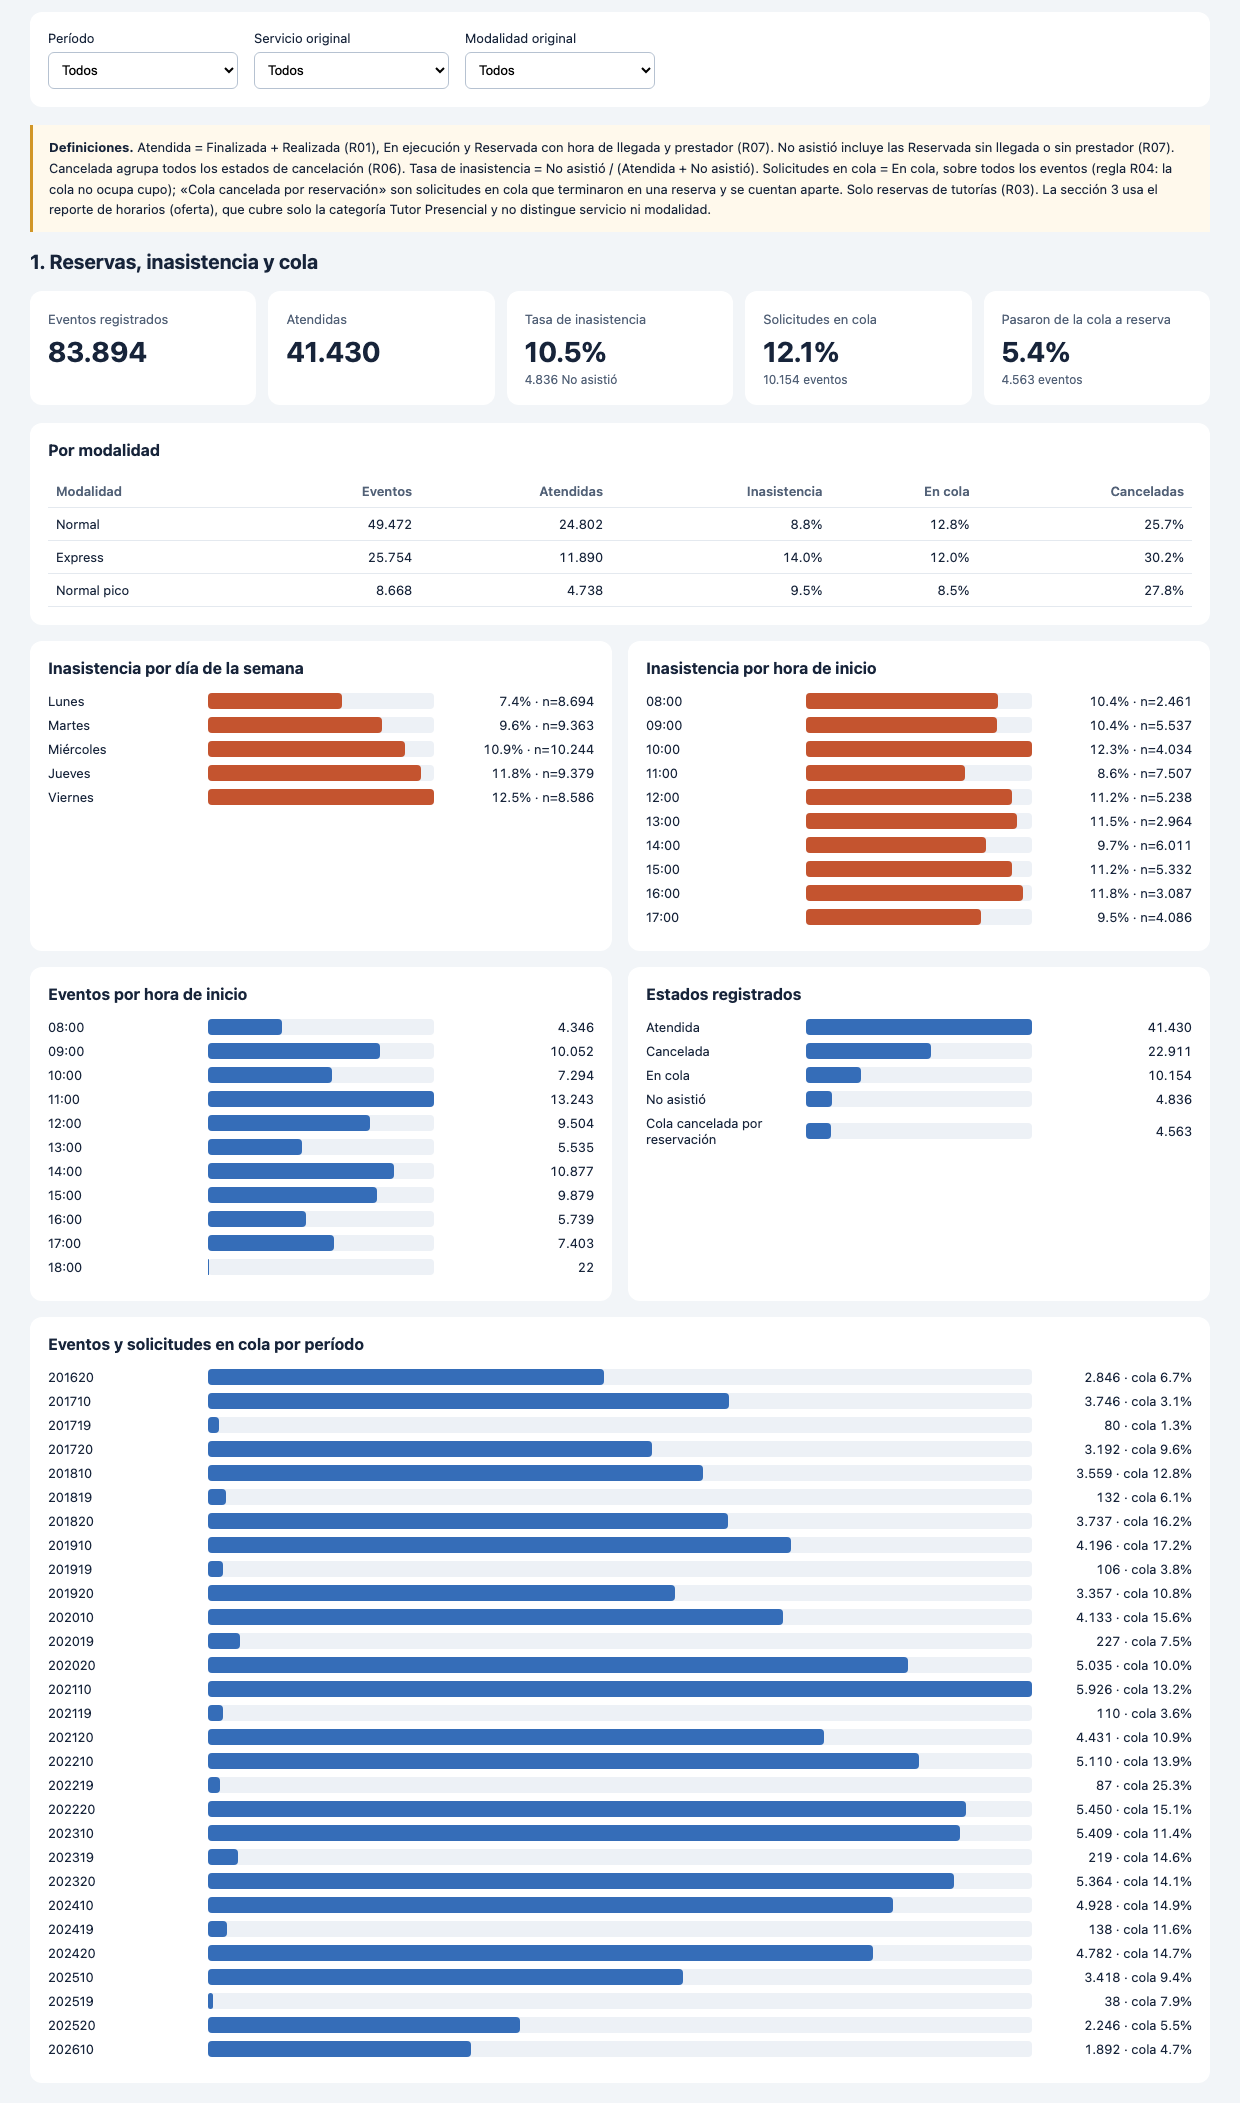
\includegraphics[width=\textwidth,height=0.45\textheight,keepaspectratio]{tablero_reservas.png}
\caption{Tablero, sección de reservas}
\end{figure}

La \textbf{tasa de inasistencia} es la parte de las citas en que el estudiante llegó a su hora, o debía haber llegado, y no se presentó. Se calcula como No asistió / (Atendida + No asistió). La \textbf{proporción en cola} es En cola / eventos; las solicitudes que salieron de la cola porque el estudiante consiguió una reserva se muestran aparte.

\begingroup\footnotesize\setlength{\tabcolsep}{4pt}\renewcommand{\arraystretch}{1.15}
\begin{longtable}{>{\raggedright\arraybackslash}p{\dimexpr 0.141\textwidth-2\tabcolsep\relax}>{\raggedleft\arraybackslash}p{\dimexpr 0.120\textwidth-2\tabcolsep\relax}>{\raggedleft\arraybackslash}p{\dimexpr 0.141\textwidth-2\tabcolsep\relax}>{\raggedleft\arraybackslash}p{\dimexpr 0.171\textwidth-2\tabcolsep\relax}>{\raggedleft\arraybackslash}p{\dimexpr 0.087\textwidth-2\tabcolsep\relax}>{\raggedleft\arraybackslash}p{\dimexpr 0.120\textwidth-2\tabcolsep\relax}>{\raggedleft\arraybackslash}p{\dimexpr 0.151\textwidth-2\tabcolsep\relax}}
\toprule
\textbf{Modalidad} & \textbf{Eventos} & \textbf{Atendidas} & \textbf{Inasistencia} & \textbf{En cola} & \textbf{Cola a reserva} & \textbf{Canceladas} \\
\midrule
\endhead
Normal & 49.472 & 24.802 & 8,8\% & 12,8\% & 6,6\% & 25,7\% \\
Express & 25.754 & 11.890 & \textbf{14,0\%} & 12,0\% & 4,0\% & 30,2\% \\
Normal pico & 8.668 & 4.738 & 9,5\% & 8,5\% & 3,3\% & 27,8\% \\
\textbf{Total} & \textbf{83.894} & \textbf{41.430} & \textbf{10,5\%} & \textbf{12,1\%} & \textbf{5,4\%} & \textbf{27,3\%} \\
\bottomrule
\end{longtable}
\endgroup


\textbf{Hallazgos:}

\begin{itemize}[leftmargin=1.5em,itemsep=2pt]
\item \textbf{Express tiene una inasistencia cerca de 60\% mayor que Normal} (14,0\% frente a 8,8\%). Como la cita es corta y fácil de reservar, el estudiante pierde poco si no llega. Es el primer candidato para recordatorios automáticos o para que la sanción también cuente en Express.
\item \textbf{La inasistencia crece a lo largo de la semana:} lunes 7,4\%, martes 9,6\%, miércoles 10,9\%, jueves 11,8\%, viernes 12,5\%. Por hora de inicio (horas con 30 o más citas), las de 10:00 (12,3\%) y 16:00 (11,8\%) son las más altas y la de 11:00 la más baja (8,6\%).
\item \textbf{Una de cada ocho solicitudes (12,1\%) queda en cola} sin conseguir cita, y otro 5,4\% sale de la cola porque consigue una reserva. La cola más alta es en Normal (12,8\%). La proporción en cola estuvo entre 10\% y 17\% de 2018 a 2024 (con un máximo de 17,2\% en 201910) y bajó a 9,4\%, 5,5\% y 4,7\% en 202510, 202520 y 202610, a la vez que el volumen de reservas cayó de unas 5.400 por semestre (202220 y 202310) a 1.892 en 202610. La coordinación debería averiguar la causa de esa caída.
\end{itemize}

\subsection{Análisis 2 · Satisfacción}

\begin{figure}[H]\centering
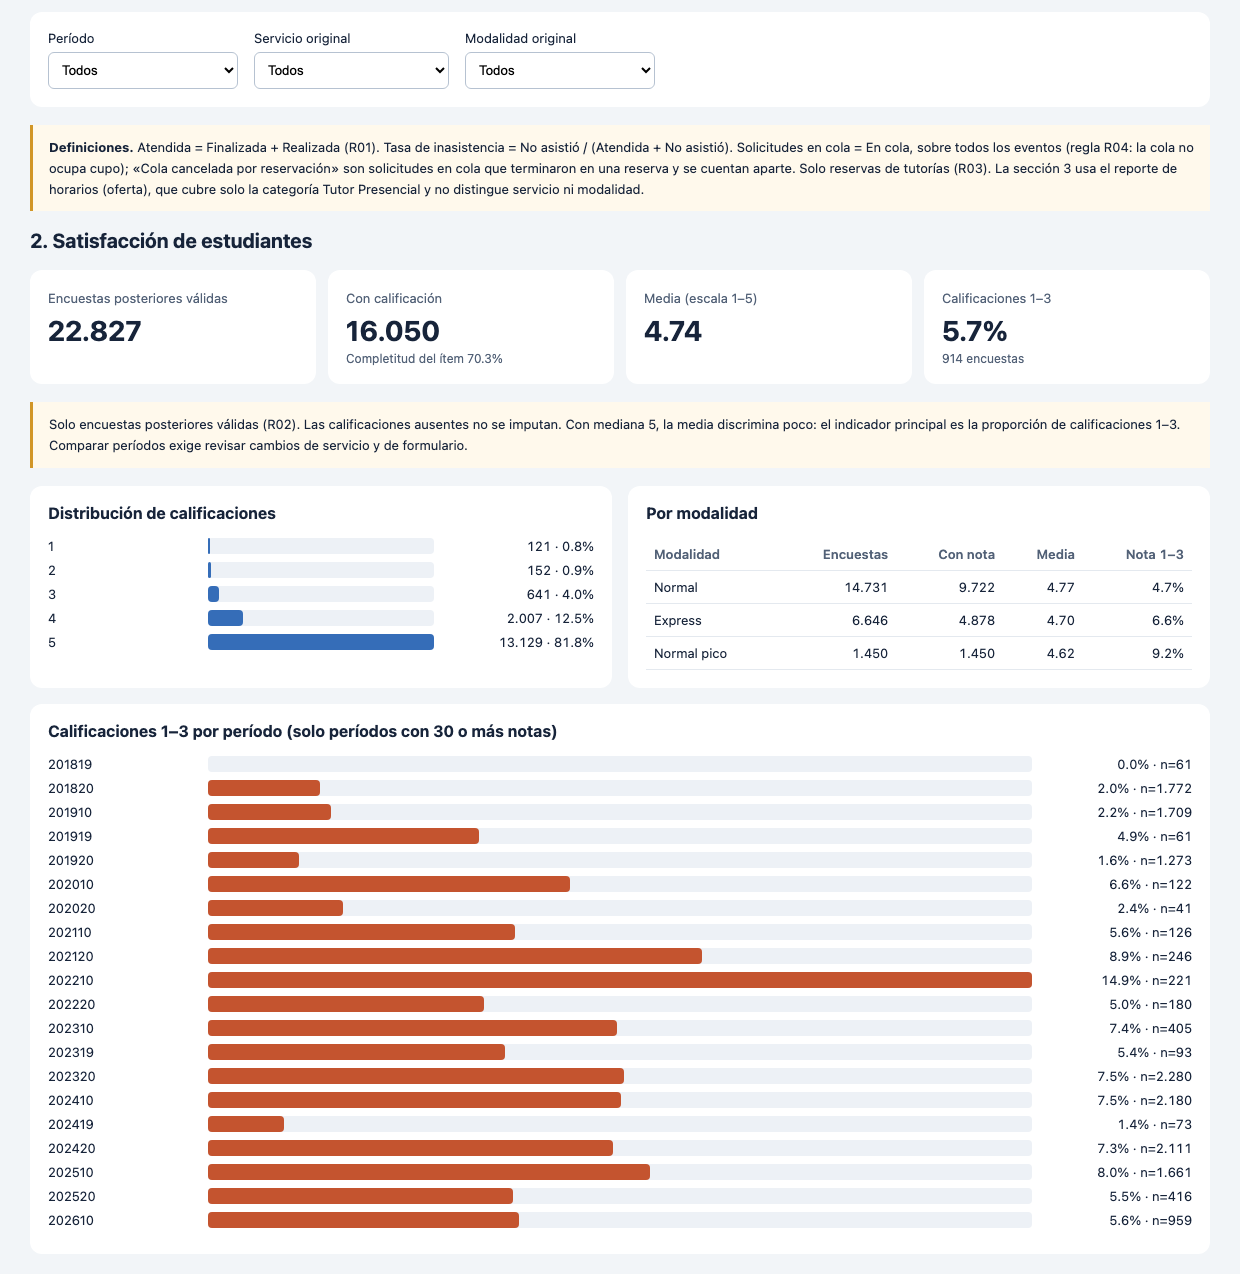
\includegraphics[width=\textwidth,height=0.45\textheight,keepaspectratio]{tablero_satisfaccion.png}
\caption{Tablero, sección de satisfacción}
\end{figure}

\begingroup\small\setlength{\tabcolsep}{4pt}\renewcommand{\arraystretch}{1.15}
\begin{longtable}{>{\raggedright\arraybackslash}p{\dimexpr 0.286\textwidth-2\tabcolsep\relax}>{\raggedleft\arraybackslash}p{\dimexpr 0.231\textwidth-2\tabcolsep\relax}>{\raggedleft\arraybackslash}p{\dimexpr 0.141\textwidth-2\tabcolsep\relax}>{\raggedleft\arraybackslash}p{\dimexpr 0.273\textwidth-2\tabcolsep\relax}}
\toprule
\textbf{Segmento} & \textbf{Calificadas} & \textbf{Media} & \textbf{Calificaciones 1 a 3} \\
\midrule
\endhead
Normal & 9.722 & 4,77 & 4,7\% \\
Express & 4.878 & 4,70 & 6,6\% \\
Normal pico & 1.450 & 4,62 & \textbf{9,2\%} \\
IP & 8.908 & 4,68 & 7,2\% \\
EDA & 2.143 & 4,69 & 7,9\% \\
APO 1 (histórico) & 4.220 & 4,86 & 2,0\% \\
\textbf{Total} & \textbf{16.050} & \textbf{4,74} & \textbf{5,7\%} \\
\bottomrule
\end{longtable}
\endgroup


\textbf{Hallazgos:}

\begin{itemize}[leftmargin=1.5em,itemsep=2pt]
\item La satisfacción es alta (media 4,74; 81,8\% de cincos). La señal útil está en el 5,7\% de calificaciones de 1 a 3.
\item \textbf{Normal pico tiene casi el doble de calificaciones bajas que Normal} (9,2\% frente a 4,7\%). Es coherente con una sesión en semana de alta demanda: más carga para el monitor y menos tiempo por estudiante.
\item \textbf{Las calificaciones bajas pasaron de cerca del 2\% (2018 y 2019, APO) a cerca del 7,5\% (2023 a 2025, IP y EDA)}, con un máximo de 14,9\% en 202210. El cambio coincide con la transición de APO a IP y con cambios en el formulario. No lo atribuimos solo al servicio, pero es el período que la coordinación académica debería revisar primero.
\item La completitud de la pregunta de calificación es del 70,3\%. Como la encuesta es voluntaria, los resultados describen a quienes respondieron.
\end{itemize}

\subsection{Por qué el modelo es adecuado para estos análisis}

\begingroup\small\setlength{\tabcolsep}{4pt}\renewcommand{\arraystretch}{1.15}
\begin{longtable}{>{\raggedright\arraybackslash}p{\dimexpr 0.465\textwidth-2\tabcolsep\relax}>{\raggedright\arraybackslash}p{\dimexpr 0.465\textwidth-2\tabcolsep\relax}}
\toprule
\textbf{Criterio} & \textbf{Cómo lo cumple el modelo} \\
\midrule
\endhead
Cada indicador se calcula sobre una sola tabla de hechos, a la granularidad correcta & Inasistencia y cola: un conteo (\texttt{COUNT}) sobre \texttt{hecho\_\allowbreak{}reserva} agrupado por \texttt{dim\_\allowbreak{}estado}. Calificaciones: \texttt{hecho\_\allowbreak{}encuesta} filtrado a la encuesta posterior. Ningún indicador cruza dos tablas de hechos fila a fila. \\
Los filtros son coherentes entre los dos análisis & Fecha (con su período), servicio y modalidad son dimensiones compartidas: el mismo filtro significa lo mismo en ambas secciones. \\
Los denominadores son explícitos & Las reglas R01, R04, R06 y R07 son atributos de la dimensión Estado (\texttt{estado\_\allowbreak{}analitico}, \texttt{grupo\_\allowbreak{}estado}) y R02 y R03 son filtros de carga; las consultas solo agrupan por esos atributos. El tablero muestra el número de casos (\emph{n}) junto a cada porcentaje. \\
Se puede pasar del resumen al detalle & Las jerarquías permiten ir de tipo de período a período, de franja a hora y de grupo de estado a estado original. Por ejemplo, la proporción en cola es 9,4\% en intersemestrales frente a 12,3\% y 12,0\% en los semestres 1 y 2. \\
El tablero no tiene que corregir problemas de calidad & Las exclusiones e inconsistencias se resuelven en Silver y Gold; el tablero solo suma y agrupa. \\
El modelo puede crecer & La oferta ya entró como una tabla de hechos propia (\texttt{hecho\_\allowbreak{}oferta}) con dimensiones compartidas (Período, Hora); la oferta por fecha concreta se incorporaría de la misma forma, y el texto ya está en \texttt{hecho\_\allowbreak{}respuesta}. \\
\bottomrule
\end{longtable}
\endgroup


\subsection{Oferta y ocupación}

\begin{figure}[H]\centering
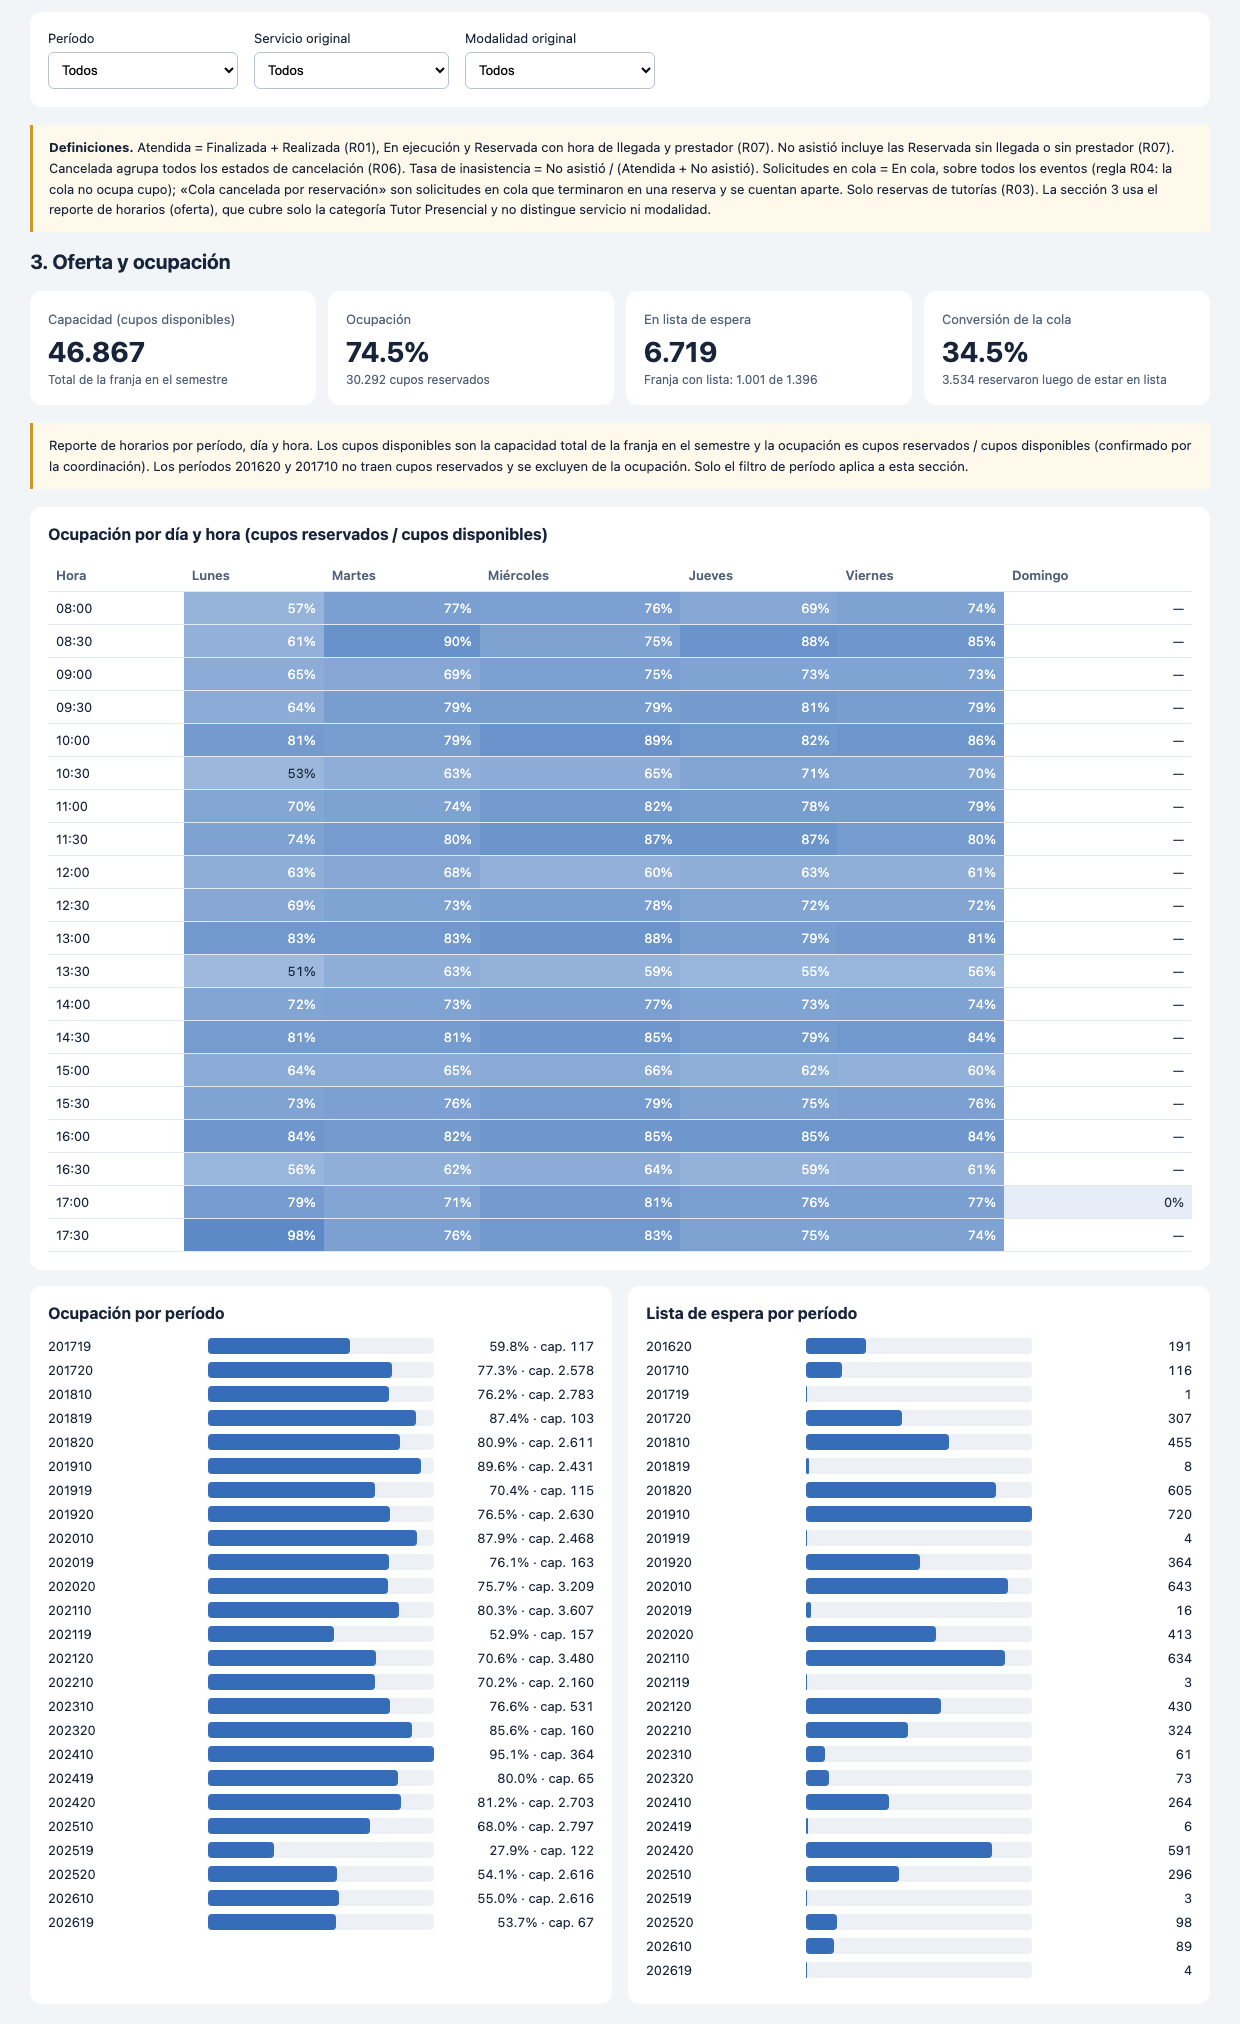
\includegraphics[width=\textwidth,height=0.8\textheight,keepaspectratio]{tablero_oferta.png}
\caption{Tablero, sección de oferta}
\end{figure}

La tercera sección del tablero usa los horarios (categoría Tutor Presencial, regla R05). Los cupos disponibles son la capacidad total de la franja en el semestre y la ocupación es cupos reservados / cupos disponibles (confirmado por la coordinación). Se excluyen de la ocupación 201620 y 201710, que no traen cupos reservados. La última columna indica qué parte de las atenciones de tutorías de cada semestre cubren los horarios.

\begingroup\footnotesize\setlength{\tabcolsep}{4pt}\renewcommand{\arraystretch}{1.15}
\begin{longtable}{>{\raggedright\arraybackslash}p{\dimexpr 0.115\textwidth-2\tabcolsep\relax}>{\raggedleft\arraybackslash}p{\dimexpr 0.135\textwidth-2\tabcolsep\relax}>{\raggedleft\arraybackslash}p{\dimexpr 0.135\textwidth-2\tabcolsep\relax}>{\raggedleft\arraybackslash}p{\dimexpr 0.154\textwidth-2\tabcolsep\relax}>{\raggedleft\arraybackslash}p{\dimexpr 0.104\textwidth-2\tabcolsep\relax}>{\raggedleft\arraybackslash}p{\dimexpr 0.144\textwidth-2\tabcolsep\relax}>{\raggedleft\arraybackslash}p{\dimexpr 0.144\textwidth-2\tabcolsep\relax}}
\toprule
\textbf{Período} & \textbf{Capacidad} & \textbf{Ocupación} & \textbf{Asistencias} & \textbf{En lista de espera} & \textbf{Conversión de la cola} & \textbf{Atenciones cubiertas} \\
\midrule
\endhead
201620 & 1.969 & --- & 1.308 & 191 & 75,5\% & 100\% \\
201710 & 4.245 & --- & 2.155 & 116 & 83,3\% & 100\% \\
201720 & 2.578 & 77,3\% & 1.598 & 307 & 52,9\% & 100\% \\
201810 & 2.783 & 76,2\% & 1.746 & 455 & 22,1\% & 100\% \\
201820 & 2.611 & 80,9\% & 1.782 & 605 & 23,2\% & 100\% \\
201910 & 2.431 & 89,6\% & 1.749 & 720 & 26,6\% & 100\% \\
201920 & 2.630 & 76,5\% & 1.479 & 364 & 31,1\% & 100\% \\
202010 & 2.468 & 87,9\% & 1.818 & 643 & 25,7\% & 100\% \\
202020 & 3.209 & 75,7\% & 2.162 & 413 & 26,1\% & 75\% \\
202110 & 3.607 & 80,3\% & 2.533 & 634 & 26,4\% & 79\% \\
202120 & 3.480 & 70,6\% & 2.041 & 430 & 22,4\% & 82\% \\
202210 & 2.160 & 70,2\% & 1.060 & 324 & 17,3\% & 45\% \\
202310 & 531 & 76,6\% & 301 & 61 & 31,5\% & 12\% \\
202320 & 160 & 85,6\% & 101 & 73 & 13,1\% & 4\% \\
202410 & 364 & 95,1\% & 255 & 264 & 9,0\% & 11\% \\
202420 & 2.703 & 81,2\% & 1.754 & 591 & 24,7\% & 77\% \\
202510 & 2.797 & 68,0\% & 1.476 & 296 & 24,9\% & 82\% \\
202520 & 2.616 & 54,1\% & 1.035 & 98 & 43,7\% & 86\% \\
202610 & 2.616 & 55,0\% & 1.085 & 89 & 33,6\% & 97\% \\
\bottomrule
\end{longtable}
\endgroup


\textbf{Hallazgos:}

\begin{itemize}[leftmargin=1.5em,itemsep=2pt]
\item \textbf{La ocupación bajó en los últimos semestres con la misma oferta.} En los semestres con cobertura casi completa la ocupación estuvo entre 68\% y 90\%; en 202520 y 202610 bajó a 54\% y 55\%, con 2.616 cupos de capacidad, parecidos a los 2.703 de 202420 y los 2.797 de 202510. Los cupos reservados pasaron de 2.196 (202420) a 1.438 (202610). La oferta no se ajustó a la caída de las reservas.
\item \textbf{Hay franjas casi llenas y otras a la mitad.} Por día y hora, la ocupación va de 51\% a 98\%: el miércoles a las 10:00, 11:30 y 13:00 supera el 87\% (con capacidades de 412 a 511 cupos), mientras que el lunes a las 13:30 y a las 10:30 está en 51\% y 53\%. Es coherente con que 1.001 de las 1.396 franjas hayan tenido lista de espera. En 202520 y 202610 solo una combinación de día y hora supera el 90\%, y 30 de 65 están por debajo del 50\%.
\item \textbf{Un tercio de la cola termina en reserva.} El 34,5\% de las solicitudes en lista (3.534 de 10.253) terminó en una reserva; en 202520 fue 43,7\% y en 202610, 33,6\%.
\item \textbf{Las inasistencias casi igualan a la lista de espera.} En los semestres 202510, 202520 y 202610 hubo 414 inasistencias y 483 solicitudes en lista, y en 54 de las 135 franjas con lista (40\%) las inasistencias alcanzaban para atenderla (214 de 1.001, el 21\%, en todo el período). La comparación es agregada y no casa fechas, pero sugiere que los recordatorios podrían absorber buena parte de la cola.
\item \textbf{Entre 202210 y 202410 las cifras de oferta no son comparables.} Los horarios cubren de 4\% a 45\% de las atenciones de esos semestres porque la mayoría de las tutorías se registró en otras categorías, y en 202220 no hay franjas.
\item \textbf{Calificación y saturación (exploratorio).} Las calificaciones de 1 a 3 son 5,8\% en el tercil de menor ocupación de la franja (hasta 69\%; 2.150 calificaciones), 4,7\% en el intermedio (de 69\% a 85\%; 3.909) y 3,3\% en el de mayor ocupación (más de 85\%; 4.230). No se confirma que las franjas más ocupadas tengan notas más bajas; la diferencia refleja sobre todo el período (los semestres de 2018 y 2019 tuvieron ocupación alta, de 76\% a 90\%, y pocas notas bajas) y no permite concluir una causa.
\end{itemize}

\subsection{Usuarios y funcionalidad del tablero}

\begingroup\small\setlength{\tabcolsep}{4pt}\renewcommand{\arraystretch}{1.15}
\begin{longtable}{>{\raggedright\arraybackslash}p{\dimexpr 0.199\textwidth-2\tabcolsep\relax}>{\raggedright\arraybackslash}p{\dimexpr 0.134\textwidth-2\tabcolsep\relax}>{\raggedright\arraybackslash}p{\dimexpr 0.299\textwidth-2\tabcolsep\relax}>{\raggedright\arraybackslash}p{\dimexpr 0.299\textwidth-2\tabcolsep\relax}}
\toprule
\textbf{Usuario} & \textbf{Análisis} & \textbf{Interacción} & \textbf{Cómo lo soporta el modelo} \\
\midrule
\endhead
Coordinación de CupiTaller & 1. Inasistencia, cola y oferta & Filtra por período, servicio y modalidad; lee las tasas con su número de casos; compara por día de la semana y hora; revisa la ocupación y la lista de espera por franja & \texttt{hecho\_\allowbreak{}reserva} con \texttt{dim\_\allowbreak{}estado} (grupo de estado), \texttt{dim\_\allowbreak{}fecha} y \texttt{dim\_\allowbreak{}hora}; \texttt{hecho\_\allowbreak{}oferta} con \texttt{dim\_\allowbreak{}periodo}, \texttt{dim\_\allowbreak{}dia\_\allowbreak{}semana} y \texttt{dim\_\allowbreak{}hora} \\
Coordinación académica de los cursos & 2. Satisfacción & Filtra por los mismos criterios; revisa la proporción de calificaciones de 1 a 3 y su evolución por período & \texttt{hecho\_\allowbreak{}encuesta} filtrado a la encuesta posterior, con dimensiones compartidas \\
Ambos & Exploración & Pasan de tipo de período a período, de franja a hora y de grupo de estado a estado original & Jerarquías guardadas en las dimensiones (4.2) \\
\bottomrule
\end{longtable}
\endgroup


El tablero no necesita servidor porque la coordinación no tiene infraestructura de BI. Las decisiones de modelo que lo hacen posible (dimensiones compartidas, reglas guardadas en \texttt{dim\_\allowbreak{}estado}, una sola granularidad por tabla de hechos) están justificadas en 4.4 y 6.3.


\section{Gestión del proyecto}

\subsection{Contribuciones y distribución de puntos}

\begingroup
\small
\setlength{\tabcolsep}{4pt}
\renewcommand{\arraystretch}{1.15}

\begin{longtable}{
>{\raggedright\arraybackslash}p{\dimexpr 0.180\textwidth-2\tabcolsep\relax}
>{\raggedright\arraybackslash}p{\dimexpr 0.752\textwidth-2\tabcolsep\relax}
>{\raggedleft\arraybackslash}p{\dimexpr 0.068\textwidth-2\tabcolsep\relax}
}
\toprule
\textbf{Integrante} &
\textbf{Trabajo realizado} &
\textbf{Puntos (de 100)} \\
\midrule
\endhead

María Alejandra Pérez Petro &
Descarga y extracción de los datos de la fuente (reservas, encuestas y horarios). Conciliación de las dudas con el coordinador de CupiTaller: significado de los estados, reglas de negocio y oferta. Documentación del proyecto y del informe. Diseño del modelo dimensional, con Santiago. &
50 \\

Santiago Martinez Novoa &
Diseño de los tableros. Arquitectura del repositorio. Apoyo en la implementación de la limpieza y la carga de datos en Gold, y creación de las consultas SQL. Diseño del modelo dimensional, con María Alejandra. &
50 \\

\bottomrule
\end{longtable}
\endgroup

La distribución es de 50 puntos para cada integrante, y suma 100. 

\textbf{Problemas identificados en el equipo:} las definiciones de la coordinación llegaron mientras ya se modelaba (la cola no ocupa cupo, el alcance a reservas de tutorías, el significado de «Cola cancelada por reservación» y los horarios de oferta), por lo que el modelo, las cifras y los tableros se recalcularon varias veces.

\textbf{Estrategias para la Entrega 2:} preguntar con mayor tiempo a la coordinación cualquier duda con respecto al significado de los datos y las reglas de negocio. Proponer analisis que permitan aprovechar la información en texto libre, como son las respuestas a las preguntas abiertas de la encuesta y los comentarios de los estudiantes en la reserva.
\subsection{Uso de inteligencia artificial generativa}

\textbf{Uso dado.} Usamos un asistente de programación con inteligencia artificial generativa para tres tareas: (i) escribir los programas que leen los archivos de Excel, perfilan los datos (calculan sus estadísticas), los limpian y los cargan en la capa Gold; (ii) generar el tablero; y (iii) revisar detalles del modelo dimensional. El diseño del modelo dimensional fue obra del equipo; la herramienta solo apoyó su revisión.

\end{document}